%!TEX encoding = UTF-8 Unicode
% ================================================================================
\documentclass[
    fontsize=12pt,
    headings=small,
    parskip=half,           % Ersetzt manuelles Setzen von parskip/parindent.
    bibliography=totoc,
    numbers=noenddot,       % Entfernt den letzten Punkt der Kapitelnummern.
    open=any,               % Kapitel kann auf jeder Seite beginnen.
%   final                   % Entfernt alle todonotes und den Entwurfstempel.
    ]{scrreprt}
% ===================================Praeambel==================================
% Kodierung, Sprache, Patches {{{
\usepackage[T1]{fontenc}    % Ausgabekodierung; ermöglicht Akzente und Umlaute
                            %  sowie korrekte Silbentrennung.
\usepackage[utf8]{inputenc} % Erlaubt die direkte Eingabe spezieller Zeichen;
                            %  utf8 muss die Eingabekodierung des Editors sein.
\usepackage[ngerman]{babel} % Deutsche Sprachanpassungen (z.B. Überschriften).
\usepackage{microtype}      % Optimale Randausrichtung und Skalierung.
\usepackage[
    autostyle,
    ]{csquotes}             % Korrekte Anführungszeichen in der Literaturliste.
%\usepackage{fixltx2e}      % Patches fuer LaTeX2e - seit 2015 nicht mehr nötig
\usepackage{scrhack}        % Verhindert Warnungen mit älteren Paketen.
\usepackage[
  newcommands
]{ragged2e}                 % Verbesserte \ragged...Befehle
\PassOptionsToPackage{
  hyphens
}{url}                      % Sorgt für URL-Umbrüche in Fußzeilen u. Literatur
% }}}

% Schriftarten {{{
\usepackage{mathptmx}       % Times; modifies the default serif and math fonts
\usepackage[scaled=.92]{helvet}% modifies the sans serif font
\usepackage{courier}        % modifies the monospace font
% }}}

% Biblatex {{{
\usepackage[
    style=alphabetic,
    backend=biber,
    %backref=true
    ]{biblatex}             % Biblatex mit alphabetischem Style und biber.
\bibliography{\jobname.bib} % Dateiname der bib-Datei.
\DeclareFieldFormat*{title}{
    \mkbibemph{#1}}         % Make titles italics
% }}}

% Dokument- und Texteinstellungen {{{
\usepackage[
    a4paper,
    margin=2.54cm,
    marginparwidth=2.0cm,
    footskip=1.0cm
    ]{geometry}             % Ersetzt 'a4wide'.
\clubpenalty=10000          % Keine Einzelzeile am Beginn eines Absatzes
                            %  (Schusterjungen).
\widowpenalty=10000         % Keine Einzelzeile am Ende eines Absatzes
\displaywidowpenalty=10000  %  (Hurenkinder).
\usepackage{floatrow}       % Zentriert alle Floats
\usepackage{ifdraft}        % Ermöglicht \ifoptionfinal{true}{false}
\pagestyle{plain}           % keine Kopfzeilen
% \sloppy                    % großzügige Formatierungsweise
\deffootnote{1em}{1em}{
  \thefootnotemark.\ }      % Verbessert Layout mehrzeiliger Fußnoten

\makeatletter
\AtBeginDocument{%
    \hypersetup{%
        pdftitle = {\@title},
        pdfauthor  = \@author,
    }
}
\makeatother
% }}}

% Weitere Pakete {{{
\usepackage{verbatim}
\usepackage{tikz}			% Für die Baumstruktur
\usetikzlibrary{positioning}
\usepackage[edges]{forest}
\usepackage{enumitem}        % style nextline für description
\usepackage{graphicx}       % Einfügen von Graphiken.
\usepackage{tabu}           % Einfügen von Tabellen.
\usepackage{multirow}       % Tabellenzeilen zusammenfassen.
\usepackage{multicol}       % Tabellenspalten zusammenfassen.
\usepackage{booktabs}       % Schönere Tabellen (\toprule\midrule\bottomrule).
\usepackage[nocut]{thmbox}  % Theorembox bspw. für Angreifermodell.
\usepackage{amsmath}        % Erweiterte Handhabung mathematischer Formeln.
\usepackage{amssymb}        % Erweiterte mathematische Symbole.
\usepackage{rotating}
\usepackage[
    printonlyused
    ]{acronym}              % Abkürzungsverzeichnis
\usepackage[
    colorinlistoftodos,
    textsize=tiny,          % Notizen und TODOs - mit der todonotes.sty von
    \ifoptionfinal{disable}{}%  Benjamin Kellermann ist das Package "changebar"
    ]{todonotes}            %  bereits integriert.
\usepackage[
    breaklinks,
    hidelinks,
    pdfdisplaydoctitle,
    pdfpagemode = {UseOutlines},
    pdfpagelabels,
    ]{hyperref}             % Sprungmarken im PDF. Lädt das URL-Paket.
    \urlstyle{rm}           % Entfernt die Formattierung von URLs.
%\usepackage{breakurl}
%\def\UrlBreaks{\do\/\do-}
\usepackage{listings}       % Spezielle Umgebung für Quelltextformatierung.
    \lstset{                
        language=csh,
        breaklines=true,
        breakatwhitespace=true,
        frame=l,            % Linie links: l, doppelt: L
		framerule=2.5pt,    % Dicke der Linie
		rulecolor=\color{gray},% Farbe der Linie
        captionpos=b,
        xleftmargin=6ex,
        tabsize=4,
        numbers=left,
        numberstyle=\ttfamily\footnotesize,
        basicstyle=\ttfamily\footnotesize,
        keywordstyle=\bfseries\color{green!50!black},
        commentstyle=\itshape\color{magenta!90!black},
        identifierstyle=\ttfamily,
        stringstyle=\color{orange!90!black},
        showstringspaces=false,
        morekeywords={  abstract, event, new, struct,
                as, explicit, null, switch,
                base, extern, object, this,
                bool, false, operator, throw,
                break, finally, out, true,
                byte, fixed, override, try,
                case, float, params, typeof,
                catch, for, private, uint,
                char, foreach, protected, ulong,
                checked, goto, public, unchecked,
                class, if, readonly, unsafe,
                const, implicit, ref, ushort,
                continue, in, return, using,
                decimal, int, sbyte, virtual,
                default, interface, sealed, volatile,
                delegate, internal, short, void,
                do, is, sizeof, while,
                double, lock, stackalloc,
                else, long, static,
                enum, namespace, string}
        }
%\usepackage{filecontents}  % Direktes Einfügen von Dateiinhalt. Wird hier für
                            %  die Verwendung einer .bib-Datei in dieser .tex-
                            %  Datei benötigt.
% }}}

% ===================================Dokument===================================

\title{Entwicklung eines Visualisierungswerkzeuges zur Demons-
tration datenschutzfreundlicher Dokumentspeicherdienste}
\author{David Kirchhausen Monteiro}

\begin{document}

\begin{titlepage}% {{{

\includegraphics[width=6.8cm]{../pic/up-uhh-logo-u-2010-u-farbe-u-rgb.pdf}
\begin{center}\Large
	% Universität Hamburg \par
	% Fachbereich Informatik
	\vfill
	Bachelorarbeit
	\vfill
	\makeatletter
	{\Large\textsf{\textbf{\@title}}\par}
	\makeatother
	\vfill
	vorgelegt von
	\par\bigskip
	\makeatletter
	{\@author} \par
	\makeatother
	geb. am 24. Januar 1994 in Hildesheim \par
	Matrikelnummer 6530927 \par
	Studiengang Software-System-Entwicklung
	\vfill
	\makeatletter
	eingereicht am {\@date}
	\makeatother
	\vfill
	Betreuer: Maximilian Blochberger, M. Sc. \par
	Erstgutachter: Prof. Dr.-Ing. Hannes Federrath \par
	Zweitgutachter: Tilmann Stehle, M. Sc.
\end{center}
\ifoptionfinal{}{}
\end{titlepage}% }}}

\chapter*{Aufgabenstellung}

Im  Zuge  dieser  Bachelorarbeit  soll  ein  einfacher  Dokumentenspeicher  entwickelt  werden,
welcher möglichst viele Nutzerdaten erfasst und speichert. Die erfassten Daten sollen anschaulich
grafisch dargestellt werden können. Weiter sollen verschiedene Szenarien entwickelt werden,
welche aufzeigen wie eine mögliche Benutzung des Services mit und ohne der Verwendung
von datenschutzfreundlichen Methoden zum Anonymisieren von Daten aussieht. Anhand der
Szenarien soll eine grafische Auswertung Unterschiede zwischen anonymisierten Daten und
nicht anonymisierten Daten visuell sichtbar machen und die Unterschiede somit leicht zugänglich
sein.

\chapter*{Zusammenfassung}
\begin{enumerate}
\item Dokumentenspeicherdienste Vorteile (Problemstellung erläutern)
\item Mögliche Datenschutz unfreundliche Aspekte von gängigen Anbietern (Problemstellung erläutern)
\item Entwicklung des Dokumentenspeichers und der Visualisierung zur deutlich Veranschaulichung von Potentiellen Unterschieden zwischen der Verwendung von Datenschutz freundlichen Methoden zum Anonymisieren oder nicht. (Bearbeitung der Problemstellung)
\begin{enumerate}
\item Implementation des Dokumentenspeichers
\item Implementation der API zur Datenübergabe 
\item Implementation des Visualisierungswerkzeug
\item Darstellung der Szenarien zur Benutzung des Visualisierungswerkzeug
\end{enumerate}
\end{enumerate}

\tableofcontents

\chapter{Einleitung}

Dokumentenspeicherdienste sind nützliche Alltagsgegenstände, welche für private sowie kommerzielle Nutzer meist unverzichtbar sind. 
Sie bieten nicht nur den Speicherplatz für wichtige Dateien der Nutzer sondern stellen auch die Sicherheit der Dateien sicher und machen sie global jederzeit verfügbar. 
Durch die große Datensammlung dieser Dienstleister machen sie sich nicht nur selbst zu lukrativen Zielen von gezielten Angriffen (Yahoo, UBER etc.), jedoch auch die Dienstleister selber können die Daten auswerten und weitere Metadaten wie z.B. die Dateigröße oder den Autor der Datei sowie Verkehrsdaten wie z.B. die IP-Adresse oder die HTTP Header Felder über die Nutzer sammeln und weiterverwenden. 
Vor allem private Nutzer sind meist gar nicht über die Risiken und das Missbrauchspotenzial aufgeklärt, welche die Verwendung solcher Dienstleistungen mit sich bringen. 
Methoden zur Verschlüsselung oder das anonymisieren von Daten sind Benutzern meist nicht bekannt, werden von den Dienstanbietern nicht angeboten oder sind schwer umzusetzen, da es einen meist erheblichen Aufwand für die Benutzer bedeutet und Kompetenzen erfordert welche diese Benutzer nicht besitzen. 
Um genau die Risiken und Missbrauchspotenziale aufzuzeigen wird im Zuge dieser Arbeit ein Dokumentenspeicherdienst entwickelt, welcher Meta- und Verkehrsdaten der Nutzer sammelt und diese in einer visuellen Darstellung zusammenfasst. 
Zur Implementation des Dokumentenspeichers wird dabei das Microsoft ASP.NET Core Framework verwendet. 
Das Framework wird benutzt um die Webbenutzeroberfläche sowie die Web API des Dokumentenspeichers zu realisieren. 
Dazu wird das Javascript Framework Data-Driven Documents, i.d.R. d3.js genannt, zur Visualisierung der Daten verwendet. 
Der Dokumentenspeicher soll vor allem den Unterschied zwischen der Verwendung von Methoden zur Verschlüsselung oder das anonymisieren von Daten visualisieren und verwaltet dazu zwei verschiedene Datensätze, wobei eine Datenmenge ohne, und eine Datenmenge mit der Verwendung von Methoden zur Verschlüsselung oder das anonymisieren von Daten erzeugt wird. Der entstehende Unterschied der gesammelten Metadaten durch die verschiedenen Methoden führt dann zu einer Veränderung in der Visualisierung, was dann den Effekt und Nutzen der Methoden deutlich sichtbar macht.  

%\chapter{Grundlagen}

%\newpage
%\section{Terminologie}
%\begin{enumerate}
%\item HTTP-Header
%\begin{enumerate}
%\item Teil des Hypertext Transfer Protocol (HTTP)
%\item Headerblock und Headerfeld nach RFC 2616(https://tools.ietf.org/html/rfc2616)
%\end{enumerate}
%\item Geo lookup
%\begin{enumerate}
%\item eine Methodik zur Bestimmung des geografischen Standort einer IP-Adresse
%\item keine eigenen Implementation der Standortbestimmung, sondern Verwendung eines öffentlich zugänglichen Service, aus Zeit und komplexitätsgründen
%\item Patent US7752210B2
%\end{enumerate}
%\item Header Fingerprint
%\begin{enumerate}
%\item eine Methodik zur Identifikation eines Benutzers anhand der von ihm Verwendeten HTTP Header
%\item Aggregation über allen Http-Header oder einem ausgewählten Set an Headerfeldern 
%\item erzeugt Fingerprint wird gehasht und gespeichert
%\item bei übereinstimmenden Fingerprints wird angenommen das diese vom gleichen Benutzer erzeugt wurden 
%\end{enumerate}
%\end{enumerate}

%\newpage
%\section{Set A / Set B}
%
%Die angeführten DbSets FileEntryItemsA und FileEntryItemsB verfügen jeweils über Daten welche zu visualisieren sind. Dabei wird das DbSet FileEntryItemsA weiterhin als die ungeschützte Datenmenge beschrieben, da diese Datenbank nur mit Daten befüllt werden soll, bei welchen keine datenschutzfreundlichen Methoden zum anonymisieren verwendet wurden. Das DbSet FileEntryItemsB wird weiterhin als geschützte Datenmenge beschrieben, da ausschließlich Daten , welche mit Methoden zum anonymisieren hochgeladen wurden, verwendet werden sollen. Dabei sollte die geschützte und ungeschützte Datenmenge in den Zugrunde liegenden Datenmenge identisch sein und lediglich die Verwendung von Methoden zum anonymisieren die Datensätze unterscheiden, sodass die beiden Datenmenge miteinander in Hinblick auf den Effekt der Verwendung von Methoden zum anonymisieren untersucht werden können. 
%So wird im jedem beschriebenen Szenario zur Benutzung des Dokumentenspeichers angenommen das ein Benutzer eine Datei einmal ohne die Verwendung von Methoden zum anonymisieren in die ungeschützte Datenmenge via HTTP hochlädt und einmal mit der Verwendung von Methoden zum anonymisieren in die geschützte Datenmenge via HTTP hochlädt.

%Das führt dazu das bei der Auswertung der Datei durch die Verwendung oder nicht Verwendung von Methoden zum anonymisieren, die erfassten Meta-Daten sich nur durch die jeweilige Art der Methoden zum anonymisieren unterscheiden und die anschließenden Visualisierung nur diesen Unterschied darstellt und keine anderen Faktoren. 



\chapter{Grundlagen}

    \section{Verwendungszweck des Dokumentenspeichers}
%Der Dokumentenspeicher dient vor allem dazu den Vergleich zwischen den unterschiedlichen gesammelten Metadaten mit und ohne die Verwendung von datenschutzfreundlichen Methoden zum Anonymisieren von Daten. 

Der Dokumenspeicher dient vor allem dazu die gesammelten Verkehrs- und Metadaten, mit und ohne die Verwendung von datenschutzfreundlichen Methoden zum Anonymisieren von Daten, zu Vergleichen und deren Unterschiede grafisch möglichst aussagekräftig darzustellen.
Die Unterschiede in den gesammelten Daten sollen vor allem zeigen, dass durch die gesammelten Verkehr- und Metadaten es möglich ist Dateien welche vom gleichen Benutzer stammen korrekt einander zuzuordnen und das die Verwendung von datenschutzfreundlichen Methoden zum Anonymisieren von Daten dies verhindern kann.
Da die Verwendung von Authentifizierungen durch einen Benutzeraccount oder ähnliches diese Zuordnung trivialisiert, wird für diesen Dokumentenspeicher keine solche Authentifizierungen verwendet. 
Für den Dokumentenspeicher wird angenommen das alle Dateien von den Benutzern so Verschlüsselt wurden, das nur die Benutzer in der Lage sind sie wieder zu Entschlüsseln.
Daher werden alle Dateien durch kryptografische Methoden logisch getrennt in einen gemeinsamen Speicher abgelegt.

\todo{mandantenspezifische Verschlüsselung, siehe ...}
Um es zu ermöglichen die gesammelten Daten in die zu Untersuchenden Gruppen von mit und ohne Verwendung von datenschutzfreundlichen Methoden zum Anonymisieren von Daten einzuteilen.
Bietet der Dokumentenspeicher zwei verschiedene API-Endpunkte an um Dateien hoch zu laden.
Die vorgesehene Verwendung sieht also vor das zuerst eine Datenmenge an Testdaten erzeugt wird, anhand welchen ein Szenario mit verschiedenen Benutzern erstellt wird, welche verschiedene Dateien zu verschiedenen Zeitpunkte hochladen sollen. 
Im zweiten Schritt wird eine oder mehrere datenschutzfreundliche Methoden zum Anonymisieren von Daten gewählt, welche untersucht werden sollen.
Im dritten Schritt wird das Szenario einmal mit und ohne die Verwendung der gewählten Methoden zum Anonymisieren ausgeführt. 
Dabei wird sichergestellt das das durch Methoden zu Anonymisieren geschützte Szenario und das ungeschützte Szenario jeweils einen anderen API-Endpunkt ansprechen.
Der Dokumentenspeicher besitzt so zwei verschiedene Datenmengen welche sich durch das wählen oder nicht wählen einer Methoden zum Anonymisieren von Daten unterscheiden.

In dem Visualisierungstool des Dokumentenspeichers kann eine Visualiserungsoption ausgewählt werden und beliebig zwischen der geschützten Datenmenge und der ungeschützten Datenmenge gewechselt werden, sodass die Unterschiede anhand der Visualisierung der beiden Datenmengen leicht erkennbar sind.

Der Dokumentenspeicher kann aber auch zur Visualisierung von einer gemischten Datenmenge aus geschützten und ungeschützten Dateien verwendet werden. Dies wird erreicht, indem die ungeschützten und geschützten Dateien lediglich über einen API-Endpunkt hochgeladen werden.

Die Verwendung reiner Datenmengen (aus nur ungeschützten und nur geschützten Dateien) eignet sich somit, die entstehenden Unterschiede durch die Verwendung von datenschutzfreundlichen Methoden zum Anonymisieren von Daten und ohne diese zu Visualisieren und ausschließlich diese Unterschiede zu Visualisieren, da die Zugrunde liegenden Dateien sich sonst nicht unterscheiden. 
  
%Dazu werden im Dokumentenspeicher für jede Hochgeladene Datei Vehrkehrsdaten, Metadaten und die Datei selbst abgespeichert.
%Diese Daten sind die Grundlage für die Visualisierung. 
%Um die Daten ohne die Verwendung von datenschutzfreundlichen Methoden zum Anonymiseren von Daten von solchen zu trennen, welche solche Methoden benutzen, stellt der Dokumentenspeicher zwei API-Endpunkte zur Verfügung.
%Ein API-Punkt für die Verwendung von datenschutzfreundlichen Methoden zum Anonymisierne von Daten und einen ohne die Verwendung solcher Methoden.
%Die Trennung der Daten in diese Kategorien ist wichtig da für den Dokumentenspeicher angenommen wird das es keine Authentifizierung durch Benutzerkonten oder ähnlichen gibt, da diese es ermöglichen würden jede Datei anhand dieser Authentifizierung einem Benutzer zuzuordnen. 
%Genauso wird angenommen das alle Dateien der Benutzern von diesen so Verschlüsselt worden sind, das nur die jeweiligen Benutzer die Dateien wieder Entschlüsseln können.

%Diese entstehenden Unterschiede werden in der Visualisierung der Daten deutlich und veranschaulichen so den Effekt der Verwendung von datenschutzfreundlichen Methoden zum Anonymisieren von Daten.
%Die durch datenschutzfreundlichen Methoden zum Anonymisieren von Daten erzeugte Datenmenge wird folgend als geschützte Datenmenge beschrieben und nimmt an, dass mindestens eine Methoden zum Anonymisieren von Daten benutzt wurde, um diese Datenmenge zu generieren. 
%Die erzeugte Datenmenge ohne die Verwendung von datenschutzfreundlichen Methoden zum Anonymisieren wird folglich als ungeschützte Datenmenge beschreiben und nimmt an das keine Methoden zum Anonymisieren von Daten benutzt wurde% oder das zumindest keine Methoden zum Anonymisieren von Daten verwendet wurde, im Aspekt auf die Eigenschaften, die in einem gegebenen Szenario untersucht wurden.
%Der Dokumentenspeicher ist somit so konzipiert, dass ein geschützter und ein ungeschützter Datensatz angelegt werden kann. 
%Dafür wurden verschiedene API-Endpunkt implementiert, welche die Trennung der beiden Datensätze ermöglicht. 
%Es können jedoch auch geschützte und ungeschützte Daten in die gleiche Datenmenge eingespeist werden, falls dies für das zu betrachtende Szenario sinnvoll ist. 
%Die folgenden vorgestellten Szenarien trennen jedoch die geschützte Datenmenge und die ungeschützte Datenmenge und verwenden die dafür vorgesehenen API-Punkte.
%Da die geschützte und ungeschützte Datenmenge verglichen werden soll, um den Effekt der zu untersuchenden Methode zum Anonymisieren von Daten sichtbar zu machen, ist es von Vorteil wenn die verwendeten Daten zum Erzeugen der geschützten und ungeschützten Datenmenge dieselben sind und sich lediglich durch die Anonymisierung der Daten und deren Effekt unterscheiden.
%Dies stellt sicher, dass lediglich der Effekt der Methode zum Anonymisieren einen Unterschied in der Visualisierung erzeugt und keine anderen Faktoren die Visualisierung beeinflussen.
%Im ideal Fall können so, durch die Betrachtung der Visualisierung der ungeschützten Datenmenge, Relationen zwischen Dateien deutlich werden, welche darauf schließen lassen, dass diese Dateien z.B. von dem gleichen Benutzer stammen.
%Die Betrachtung der geschützten Datenmenge sollte dann im ideal Fall zeigen, dass durch die Verwendung von einer oder mehreren Methoden zum Anonymisieren von Daten diese Relation nicht mehr sichtbar ist und die Methode somit einen sichtbaren Effekt hat.

\newpage
    \section{Implementation des Dokumentenspeichers}    
    
%Der entwickelte Dokumentenspeicher besteht aus einer Controller-Klasse, welche verschiedene API-Endpunkte implementiert. 
%Die API-Endpunkte werden durch Routen angesprochen, welche vorher definiert worden. 
%Die implementierten Routen sind: 

%In der Controllerklasse ist auch für das Sammeln der Meta-Daten für die hochgeladenen Dateien zuständig und speichert diese mit Hilfe der Modellklasse in einem Datenbankschema ab. 
%Die Modellklasse besitzt verschiedene Eigenschaften, welche die gesammelten Metadaten widerspiegeln. 
%Die Eigenschaften sind : 

%Diese Eigenschaften enthalten alle gesammelten Metadaten und können zur Visualisierung verwendet werden. 
%Mit Hilfe des Entity Framework Core von Microsoft wird ein Datenbankschema erzeugt, was dieser Modellklasse entspricht. 
%Dabei wird eine SQLite Datenbankdatei erzeugt, die dem Datenbankschema entspricht und im Verzeichnis der Anwendung liegt.
%Im Gegensatz zur Verwendung eines festen SQL Server, der die Datenbank verwaltet, bietet die Anwendung so mehr Flexibilität und erlaubt es mehrere Datenbankdateien mit der Anwendung bereit zu stellen, um so verschiedene Szenarien in verschiedenen Dateien bereitzustellen.


    \subsection{Verwendete Technologien}
Der Dokumentenspeicher wurde mit Hilfe des ASP.NET Core Framework erstellt. 
Das Framework ist Microsofts aktuellste plattformübergreifendes Framework zur Realisierung von Webanwendungen.
Das Framework unterstützt alle gängigen Betriebssysteme wie Windows, Mac OS und Linux.
Mit dem ASP.NET Core entwickelte Webanwendungen lassen sich in gängige Hostingplatformen wie, z.B. das IIS von Microsoft, integrieren oder können auch in einem eigenen Prozess selbst gehostet werden. 
Das ASP.NET Framework sieht dabei eine MVC-Architektur der Projekte vor und verwenden diese Architektur intern zum Realisieren der Anwendungen. 
Modelle werden in diesem Kontext als Objekte zur Datenrepräsentation verstanden. 
Views sind die HTML-Seiten welche an die Klienten ausgegeben werden.
Controller sind zentrale Elemente. 
Sie stellen die Funktionalität von Views auf der Serverseite dar.
Sie sind zur Steuerung verschiedener Routen und die Implementation von API-endpunkten vorgesehen.
Dabei verwalten die Controller ebenfalls die zu Grunde liegenden Datenbanken.
    \subsection{Aufbau des Dokumentenspeichers}

Der entwickelt Dokumentenspeicher besteht aus aus einer Controller-Klasse, einer Modell-Klasse und drei verschiedenen View-Klassen.
Dazu eine Datenbankkontext-Klasse zur Verwaltung der Datenbank und Synchronisation zwischen Modell-Klasse und der verwendeten Datenbank.
Die Controller-Klasse implementiert verschiedene API-Endpunkte, welche das das hochladen von Dateien und die Abfrage der gesammelten Daten ermöglichen.

\begin{description}[style=nextline]   
\item[/api/GetA] HTTP Get Methode welche die gesammelten Verkehrs- und Metadaten der ungeschützten Daten ausgiebt
\item[/api/GetB] HTTP Get Methode welche die gesammelten Verkehrs- und Metadaten der geschützten Datensatz ausgiebt
\item[/api/uploadA] HTTP Post Methode zum hochladen von ungeschützten Dateien
\item[/api/uploadB] HTTP Post Methode zum hochladen von geschützten Dateien
\item[api/uploadEmu] HTTP Post Methode zum erzeugen von Dummy Daten
\end{description}

Beim hochladen der Dateien werden in der Kontroller-Klasse die Verkehrs und Metadaten der Dateien erfasst, sowie die hochgeladenen Dateien abgespeichert.
Mit Hilfe der Modellklasse werden die gesammelten Daten sowie der Pfad zu der gespeicherten Datei in der Datenbank abgelegt.

Die Modellklasse hält für alle erfassten Verkehr- und Metadaten Eigenschaften, welche diese Repräsentieren. 
 
\begin{description}[style=nextline]
\item[ID] Datenbank Index
\item[Set] Das Set bezeichnet die Gruppe welcher die Datei zugeordnet wurde
\item[Filename] Der Dateiname
\item[Filepath] Der Pfad zur gespeicherten temporären Datei
\item[Size] Die Dateigröße in Byte
\item[IPAddress] Die IP-Adresse von der die Datei hochgeladen wurde
\item[Headers] Ein String bestehend aus den Headern der Datei
\item[HeaderFingerprint] Ein Zusammenschluss aus ausgewählten Headern um eine möglichst eindeutige Signatur zu erzeugen
\item[DateTime] Als Zeitstempel für das Hochladen der Datei
\item[Country] Land aus welchem die Datei hochgeladen wurde
\item[RegionName] Region (Bundesland) aus welchem die Datei hochgeladen wurde
\item[City] Stadt aus welchem die Datei hochgeladen wurde
\item[Lat] Breitengrad welcher mit der bekannten IP-Adresse assoziiert wird
\item[Lon] Längengrad welcher mit der bekannten IP-Adresse assoziiert wird
\item[Isp] Der Internetanbieter welcher der IP zugeordnet ist
\end{description}

Der Dokumentenspeicher besitzt 3 Views, welche HTML-Seiten darstellen welche ein Benutzer über bestimme Routen aufrufen kann. 

\begin{description}[style=nextline] 
\item[/FileEntry] Anzeige der Datenbank in tabellarischer Form
\item[/FileEntryCreate] Bietet Möglichkeiten zum Hochladen von Dateien oder dem Erzeugen von Pseudodaten
\item[/FileEntryVisual] Visualisierung der gesammelten Daten
\end{description}

Die FileEntry HTML-Seite ist ist die Startseite der Webanwendung und verweist zu der FileEntryCreate und FileEntryVisual HTML-Seite.
Die FileEntry HTML-Seite zeigt lediglich die Datenbank in tabellarischer Form und ist hauptsächlich für die Entwicklung gebraucht worden. 
Dies gilt auch für die FileEntryCreate HTML-Seite. 
Die FileEntryVisual-Page ist der Hauptbestandteil dieser Arbeit und stellt die verschiedenen Visualisierungsmöglichkeiten dar.

\todo{FileEntryPage beschreiben und Funktionen zeigen}

\chapter{Hauptteil}

    \section{Beipiel: Alice und Bob}
Um die Visualisierungen an einem Beispiel zu erläutern wird ein Szenario definiert welches die Benutzung des Dokumentenspeichers und die verwendeten Daten definiert.
Dazu werden zwei Benutzer Alice und Bob definiert, welche sich beide in Hambrug befinden und sich in den Verkehrs- und Metadaten unterscheiden, sodass wir sie anhand dieser klar unterscheiden können.
Alice und Bob laden jeweils drei hypothetische Dateien mit und ohne die Verwendung einer Methode zum Anonymisieren ihrer Daten hoch.
Alice Dateien sind test0 bis test2 und Bobs Dateien sind test3 bis test5 und haben alle unterschiedliche Dateigrößen.
Die Verkehrs- und Metadaten für diese Dateien sind so gewählt das sie nicht realitätsfern sind und sich eignen die verschiedenen Visualisierungen daran aufzuzeigen. 
Es wird angenommen das die Dateien einzeln in einem Abstand von ein paar Sekunden hochgeladen werden.
Für die Verwendung einer Methode zum Anonymisieren ihrer Daten betrachten wir im 1. Fall die Verwendung eines Proxy welcher von Alice und Bob benutzt wird und im 2. Fall die Verwendung der Tor-Netzwerks. Bei der Verwendung des Tor-Netzwerks nehmen wir das für jede hochgeladene Datei eine andere Route durch das Tor-Netzwerk gewählt wird, sodass sich die Exit-Server für jede hochgeladenen Datei ändern.

Für die Benutzer nehmen wir folgende Verkehrsdaten an: 
\paragraph{Alice}
\begin{itemize}
  \item IP: 
  \begin{itemize}
  \item IP-Adresse: 95.91.226.214
  \item Lat: 53.5770988464355 Lon: 10.0190000534058
  \item Land: Deutschland Region: Hamburg Stadt: Hamburg
  \end{itemize}
  \item Headerfigerprint:  
  \begin{itemize}
  \item Accept: text/html, application/xhtml+xml, application/xml;q=0.9,*/*;q=0.8
  \item Accept-Encoding: gzip, deflate
  \item User-Agent: Mozilla/5.0 (Macintosh; Intel Mac OS X 10\_11\_6) AppleWebKit/601.7.7 (KHTML, like Gecko) Version/9.1.2 Safari/601.7.7
  \end{itemize}
\end{itemize}

\paragraph{Bob}
\begin{itemize}
  \item IP: 
  \begin{itemize}
  \item IP-Adresse: 95.91.225.215
  \item Lat: 53.5830001831055 Lon: 9.98130035400391
  \item Land: Deutschland Region: Hamburg Stadt: Hamburg
  \end{itemize}
  \item Headerfigerprint:  
  \begin{itemize}
  \item Accept: text/html, application/xhtml+xml, application/xml;q=0.9,*/*;q=0.8
  \item Accept-Encoding: gzip, deflate
  \item User-Agent: Mozilla/5.0 (Windows NT 10.0; Win64; x64; rv:60.0) Gecko/20100101 Firefox/60.0
  \end{itemize}
\end{itemize}


\newpage
    \subsection{IP-Adressen bezogene Visualisierung} \label{ipVis}
Die IP-Adressen können mit Hilfe des Dokumentenspeichers auf zwei unterschiedliche weisen Visualisiert werden. 
Einmal die Darstellung durch eine sog. TreeMap, welche eine gegebene Baumstruktur visualisieren kann. 
Und die Darstellung auf einer Karte, indem die Geo-Position einer IP-Adresse gezeigt wird.

Die Baumstruktur besteht aus einem Wurzelknoten, den davon abgehenden Kindknoten und den Blattknoten, welche dadurch ausgezeichnet sind das sie keine Kindknoten besitzen. 
Der Wurzelknoten wird künstliche erzeugt und als Überschrift für die Visualisierung verwendet und Zeigt die Schlüsseleigenschaft über dem die Baumstruktur erzeugt wurde, in diesem Fall die IP-Adresse.
Die restlichen Knoten sind aus den gegebenen Daten erzeugt worden, sodass alle Dateien mit der gleichen IP-Adresse unter einem Knoten zusammen gefasst werden.
Die erzeugte Baumstruktur hat somit 3 Ebenen. 
Auf der 1. Ebene den Wurzelknoten, welche zum Visualisieren der Schlüsseleigenschaft benutzt wird. 
Auf der 2. Ebene die Kindknoten, welche die IP-Adressen darstellen, welche im Datensatz vorhanden sind und auf der 3. Ebene die Blattknoten, welche die Dateien selbst darstellen.

In Abbildung~\ref{fig:baum} ist die erzeugte Baumstruktur für die Beispieldaten von Alice und Bob zu sehen. 
Als Wurzelknoten wird die Schlüsseleigenschaft der IP-Adresse gewählt. 
Auf der darunter liegenden Ebene sind die IP-Adresse und Alice und Bob aufgeführt.
Zu jedem dieser Knoten sind die jeweiligen Dateien der beiden Benutzer als Blattknoten angehängt.

\begin{figure}[H]
\centering
	\begin{forest}
  	for tree={%
    	folder,
    	grow'=0,
    	fit=band,
  	}
  	[Schlüsseleigenschaft: IP-Adresse
  		[Alice (95.91.226.214)
			[test0]
			[test1]
			[test2]  		
  		]
  		[Bob (95.91.225.215)
			[test3]  	
  			[test4]
  			[test5]
  		]
  	]
	\end{forest}
\caption{Baumstruktur erzeugt aus dem ungeschützten Beispieldaten von Alice und Bob}
\label{fig:baum}
\end{figure}

Aus dieser Struktur wird nun die TreeMap erzeugt. 
Für jeden Knoten im Baum wird ein Rechteck/Box erzeugt, dabei wird jeder Kindknoten in das Rechteck/Box des Elternknoten eingebettet. 
Durch farbliche Unterschiede sollen dann die verschiedenen Ebenen und Relationen deutlich werden. 
Eine Schematische Darstellung des Beispiels ist in~\ref{fig:schem} zu sehen. 

\begin{figure}[H]
\centering
\begin{tikzpicture}
\node (rect) [rectangle, draw, minimum width=160mm, minimum height=90mm, anchor= north west] at (0,0) {};
\node [below right] at (rect.north west) {Schlüsseleigenschaft: IP-Adresse};

\node (rectA) [rectangle, draw, minimum width=80mm, minimum height=80mm, anchor= north west] at (0,-1) {};
\node [below right] at (rectA.north west) {Alice (95.91.226.214};

\node (rectA0) [rectangle, draw, minimum width=22mm, minimum height=60mm, anchor= north west] at (0.35,-2) {};
\node [] at (rectA0.center) {test0};
\node (rectA1) [rectangle, draw, minimum width=22mm, minimum height=60mm, anchor= north west] at (2.9,-2) {};
\node [] at (rectA1.center) {test1};
\node (rectA2) [rectangle, draw, minimum width=22mm, minimum height=60mm, anchor= north west] at (5.45,-2) {};
\node [] at (rectA2.center) {test2};

\node (rectB) [rectangle, draw, minimum width=80mm, minimum height=80mm, anchor= north west] at (8,-1) {};
\node [below right] at (rectB.north west) {Bob (95.91.225.215)};

\node (rectB0) [rectangle, draw, minimum width=23mm, minimum height=60mm, anchor= north west] at (8.35,-2) {};
\node [] at (rectB0.center) {test3};
\node (rectB1) [rectangle, draw, minimum width=23mm, minimum height=60mm, anchor= north west] at (10.9,-2) {};
\node [] at (rectB1.center) {test4};
\node (rectB2) [rectangle, draw, minimum width=23mm, minimum height=60mm, anchor= north west] at (13.45,-2) {};
\node [] at (rectB2.center) {test5};
\end{tikzpicture}
\caption{Schematische Darstellung einer Visualitionmöglichkeit der Baumstruktur}
\label{fig:schem}
\end{figure}

In Abbildung~\ref{fig:ungIpTM} und der Abbildung~\ref{fig:ungIpM} werden die Beispieldaten von Alice und Bob mit dem Visualisierungstool des Dokumentenspeichers dargestellt.
In Abbildung~\ref{fig:ungIpTM} sind die zwei IP-Adressen von Alice(95.91.226.214) und Bob(95.91.225.215) dargestellt.
Alice sind die Dateien testo, test1 und test2 zugeordnet.
Bob sind die Dateien test3, test4 und test5 zugeordnet. 
In Abbildung~\ref{fig:ungIpM} sind zwei Standpunkte im Hamburg zu erkennen.
Den Standpunkt von Alice (Lat: Lon:) und dem Standpunkt von Bob (Lat: Lon:)

\begin{figure}[H]
%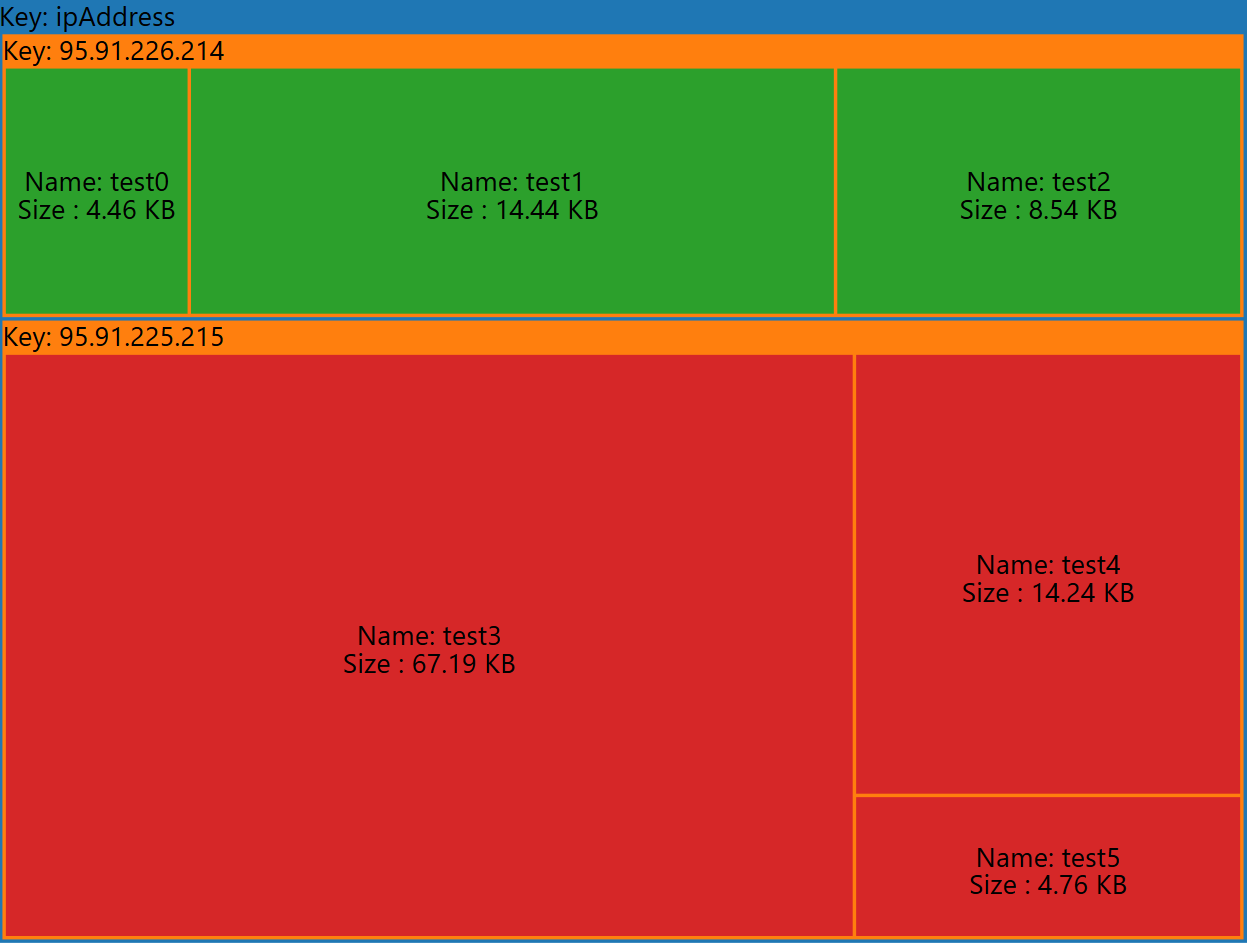
\includegraphics[width=\textwidth]{../pic/IP-Proxy-SetA-tree2.png}
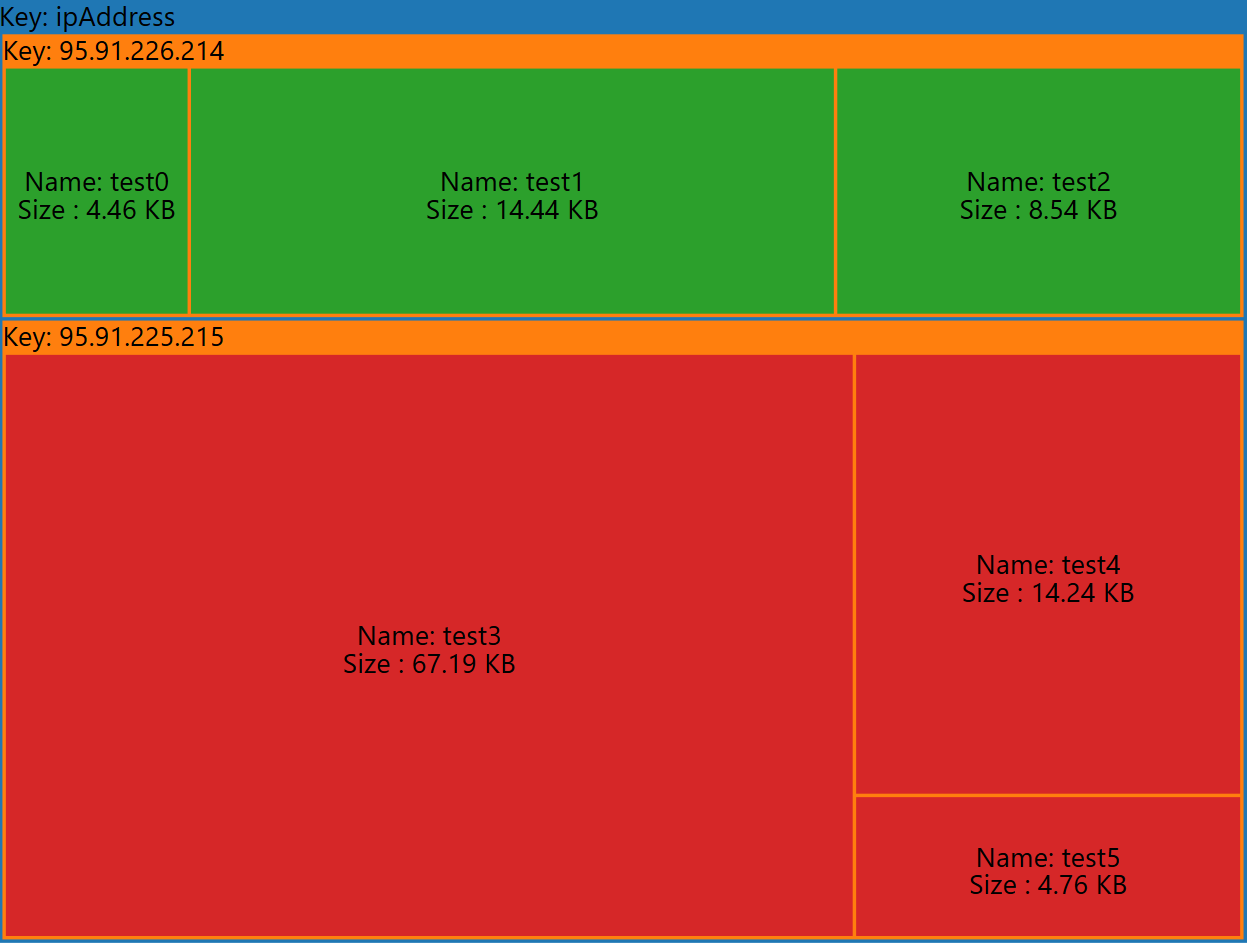
\includegraphics[width=0.7\textwidth]{../pic/IP-Proxy-SetA-tree2.PNG}
\captionof{figure}{Darstellung der ungeschützten Beispieldaten von Alice und Bob}
\label{fig:ungIpTM}
\end{figure}

\begin{figure}[H]
%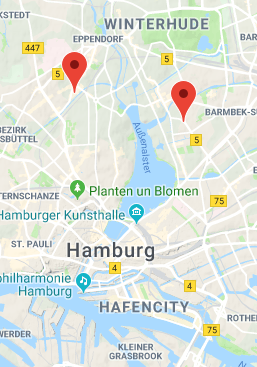
\includegraphics[width=0.5\textwidth]{../pic/IP-Proxy-SetA.png}
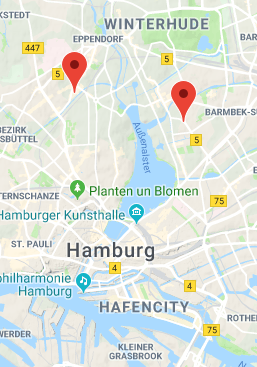
\includegraphics[width=0.5\textwidth , height=0.4\textheight]{../pic/IP-Proxy-SetA.PNG}
\captionof{figure}{Darstellung der ungeschützten Beispieldaten von Alice und Bob}
\label{fig:ungIpM}
\end{figure}

Die Darstellung der Daten spiegelt somit die definierten Beispieldaten korrekt wieder und erlaubt es die jeweiligen Daten den richtigen Benutzer zu zuordnen.


Beim Betrachten des ersten Falls, der Verwendung eines Proxys erhalten wir die Visualisierung wie in Abbildung~\ref{fig:PIpTM} und Abbildung~\ref{fig:PIpM}.
In Abbildung~\ref{fig:PIpTM} ist nur die IP-Adresse des Proxys dargestellt.
Alle definierten Dateien sind dieser IP-Adresse zugeordnet. 
In Abbildung~\ref{fig:PIpM} ist ein Standpunkt in Berlin markiert.

\begin{figure}[H]
%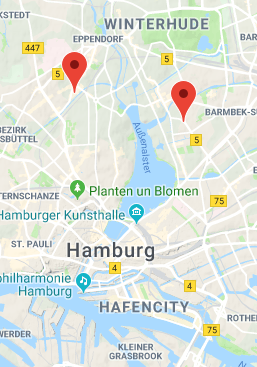
\includegraphics[width=0.5\textwidth]{../pic/IP-Proxy-SetA.png}
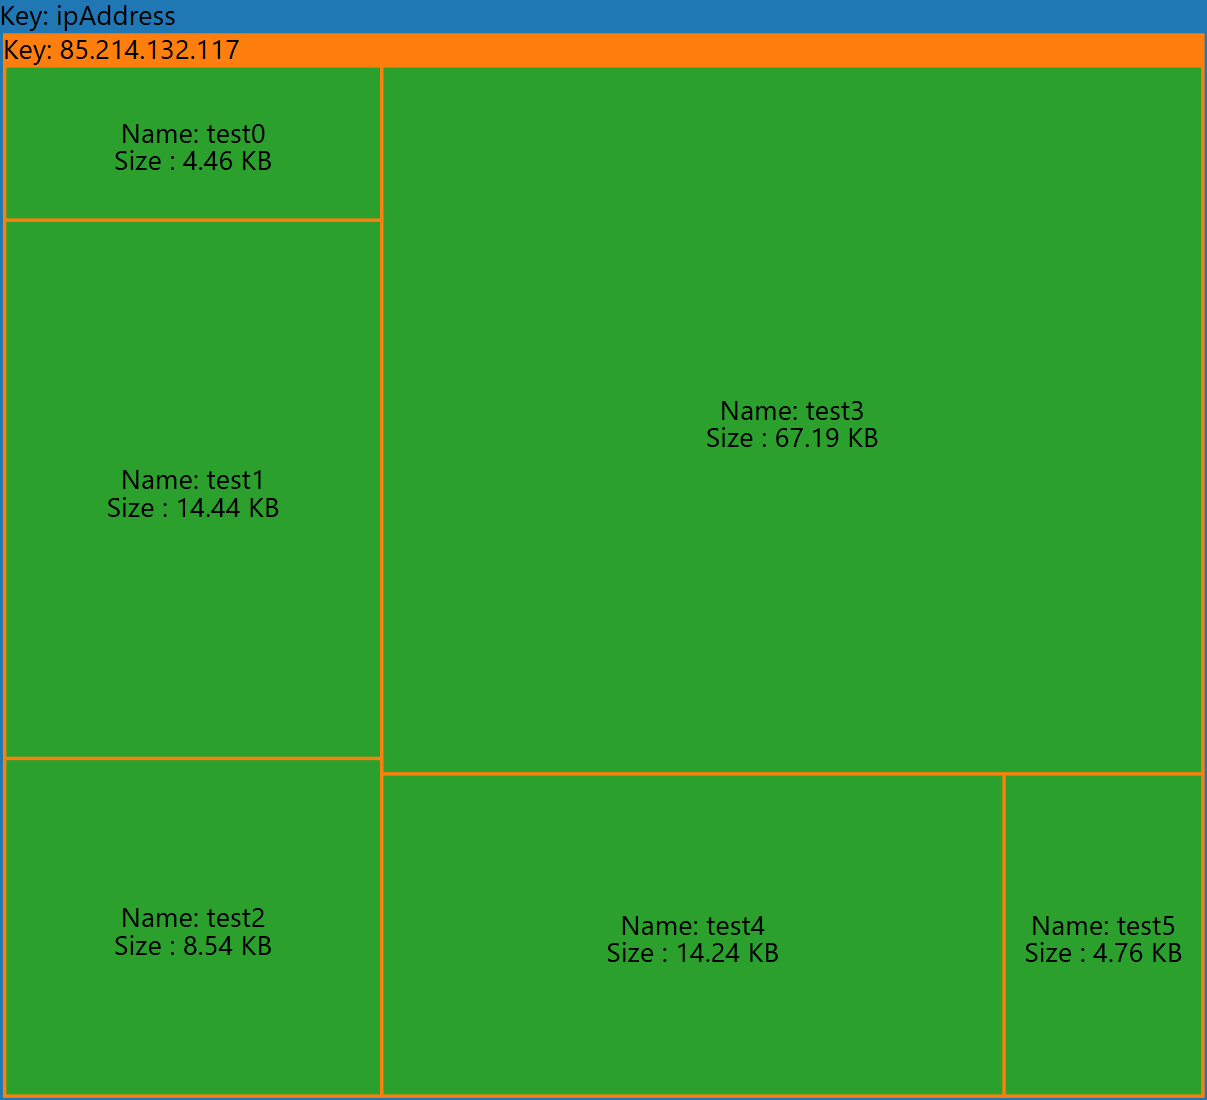
\includegraphics[width=0.7\textwidth]{../pic/IP-Proxy-SetB-tree2.PNG}
\captionof{figure}{Darstellung der Beispieldaten von Alice und Bob bei der Verwendung eines Proxys}
\label{fig:PIpTM}
\end{figure}

\begin{figure}[H]
%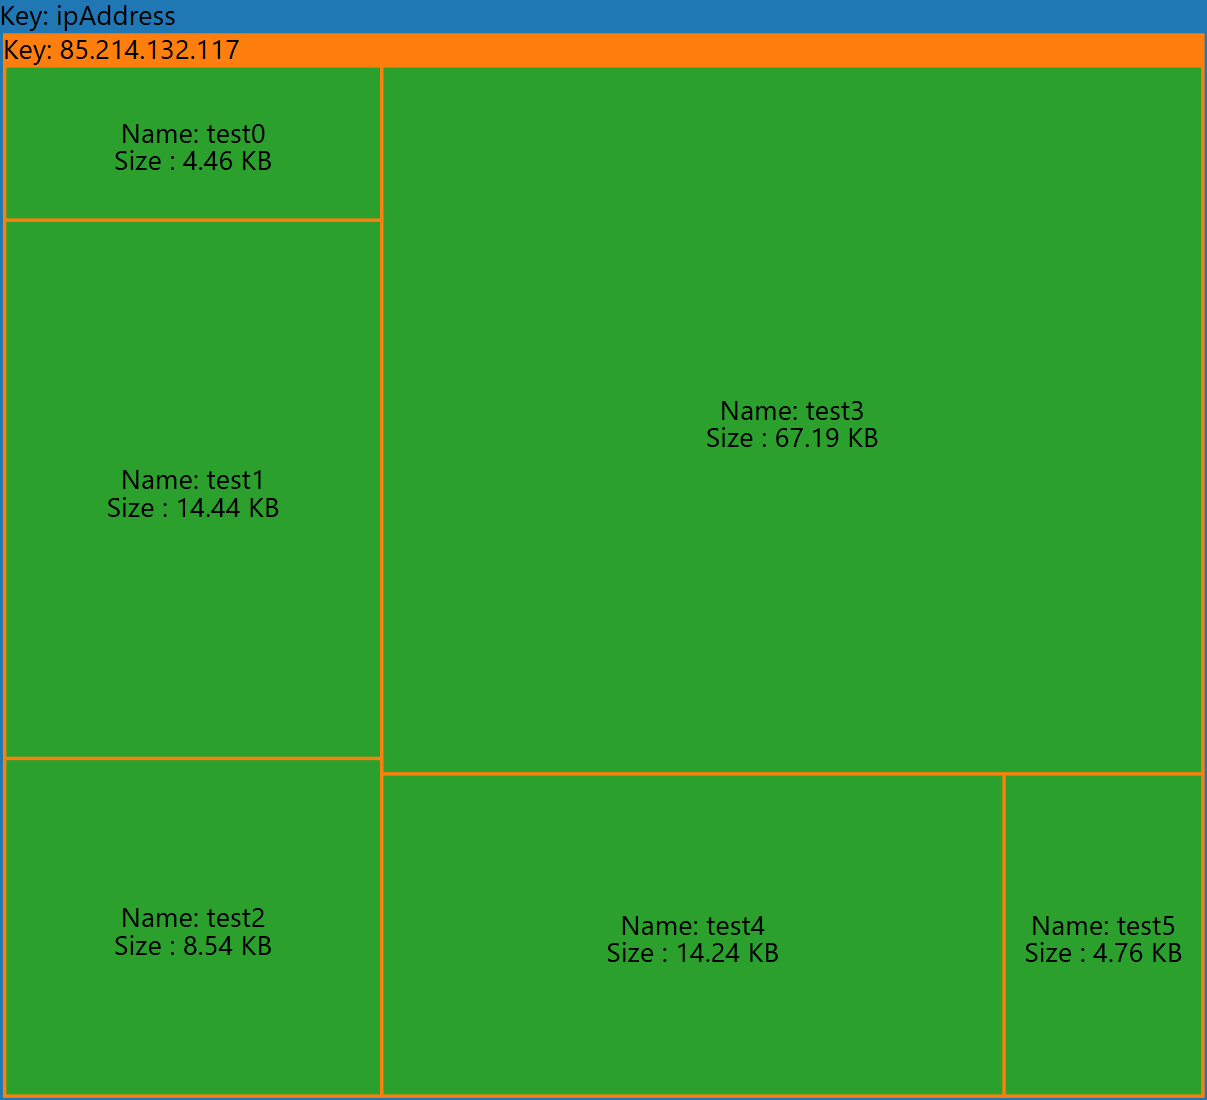
\includegraphics[width=\textwidth]{../pic/IP-Proxy-SetB-tree2.png}
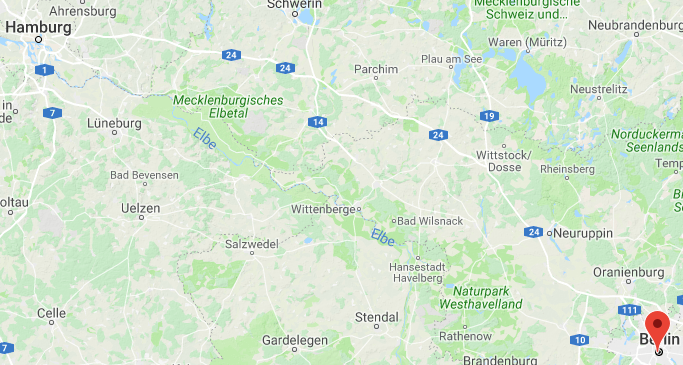
\includegraphics[width=0.5\textwidth , height=0.2\textheight]{../pic/IP-Proxy-SetB.PNG}
\captionof{figure}{Darstellung der Beispieldaten von Alice und Bob bei der Verwendung eines Proxys}
\label{fig:PIpM}
\end{figure}

Der Effekt der Proxys, welche die IP-Adressen von Alice und Bob maskiert ist in Abbildung~\ref{fig:PIpTM} klar erkennbar. Die Ip-Adressen von Alice und Bob sind nicht erkennbar und alle Dateien der beiden Benutzer der Ip-Adresse des Proxys zugeordnet. Die Dateien von Alice und Bob sind somit durch die entstandene Anonymitätsmenge geschützt, sodass wir annehmen können das die Anonymitätsmenge die Daten der beiden Benutzer enthält, die Daten aber innerhalb der Menge nicht unterschiden werden können und somit Anonymität erreicht haben. 
Im Vergleich zu den ungeschützten Daten aus der Abbildung~\ref{fig:ungIpTM}, ist die Fähgkeit anhand der IP-Adresse die Dateien genau den jeweiligen Benutzern zu zuordnen verloren gegangen, dadurch das die Benutzer einen Proxy verwendet haben.


Die entstehender Visualisierungen beim betrachten des zweiten Falls sind in Abbildung~\ref{fig:TIpTM} und Abbildung~\ref{fig:TIpM} abgebildet.

In der Abbilung~\ref{fig:TIpTM} sind 6 verschiedene IP-Adressen erkennbar.
Jeder IP-Adresse sind eine Datei zugeordnet.
\begin{description}
\centering
\item[81.7.10.29] Datei: test0
\item[129.13.131.140] Datei: test1
\item[2.202.33.28] Datei: test2
\item[81.169.133.228] Datei: test3
\item[85.197.58.203] Datei: test4
\item[178.63.80.54] Datei: test5
\end{description}

Für jede dieser IP-Adressen ist in der Karte in Abbildung~\ref{fig:TIpM} ein Standort abgebildet, welche über Deutschland verteilt sind. 
s
\begin{figure}[H]
%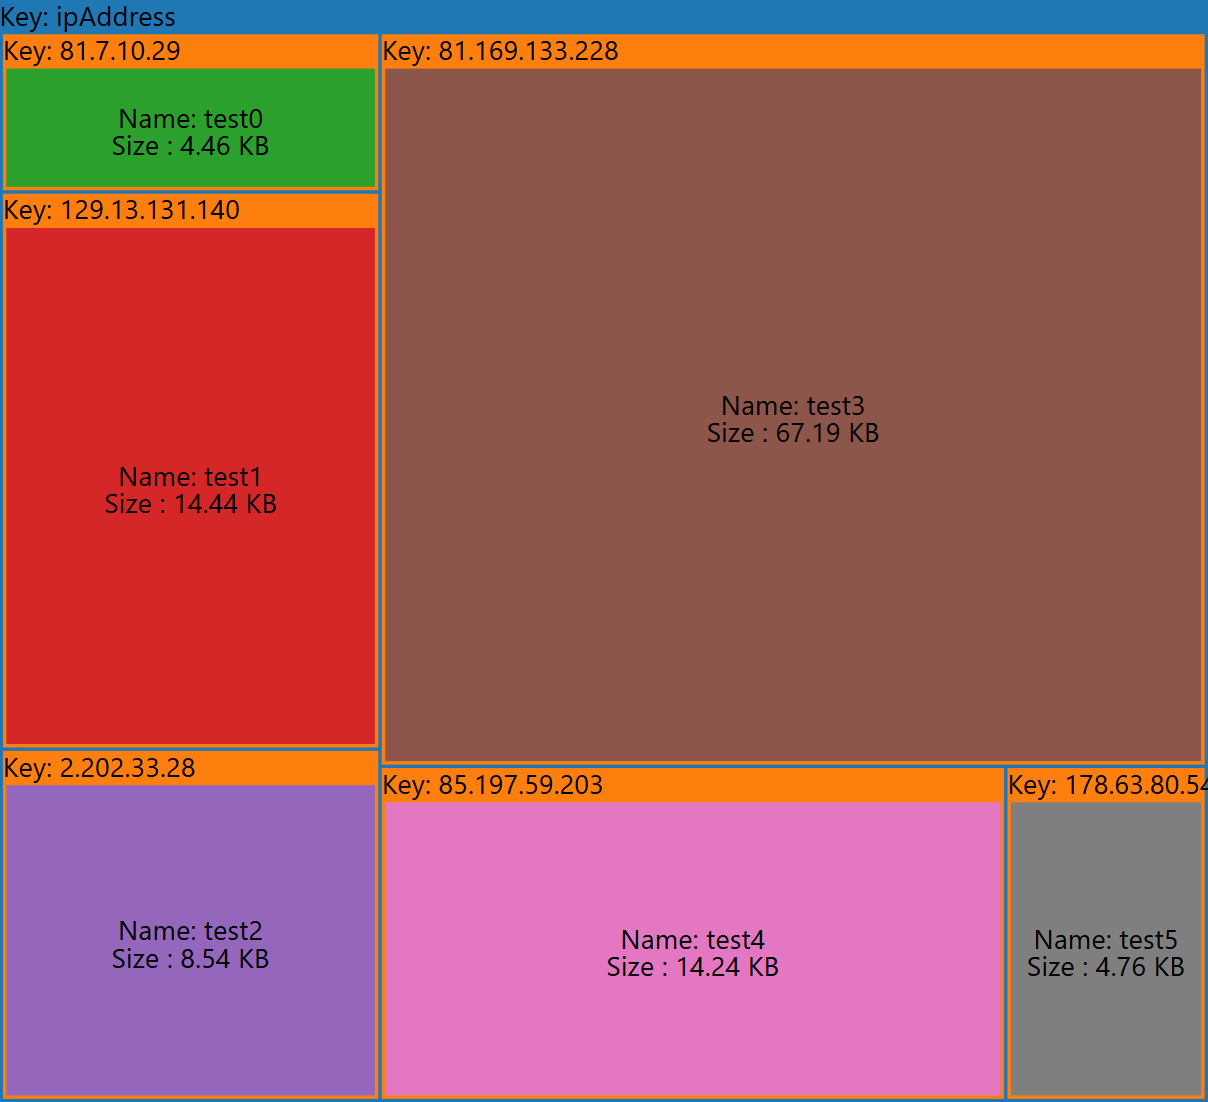
\includegraphics[width=\textwidth]{../pic/IP-Tor-SetB-tree2.png}
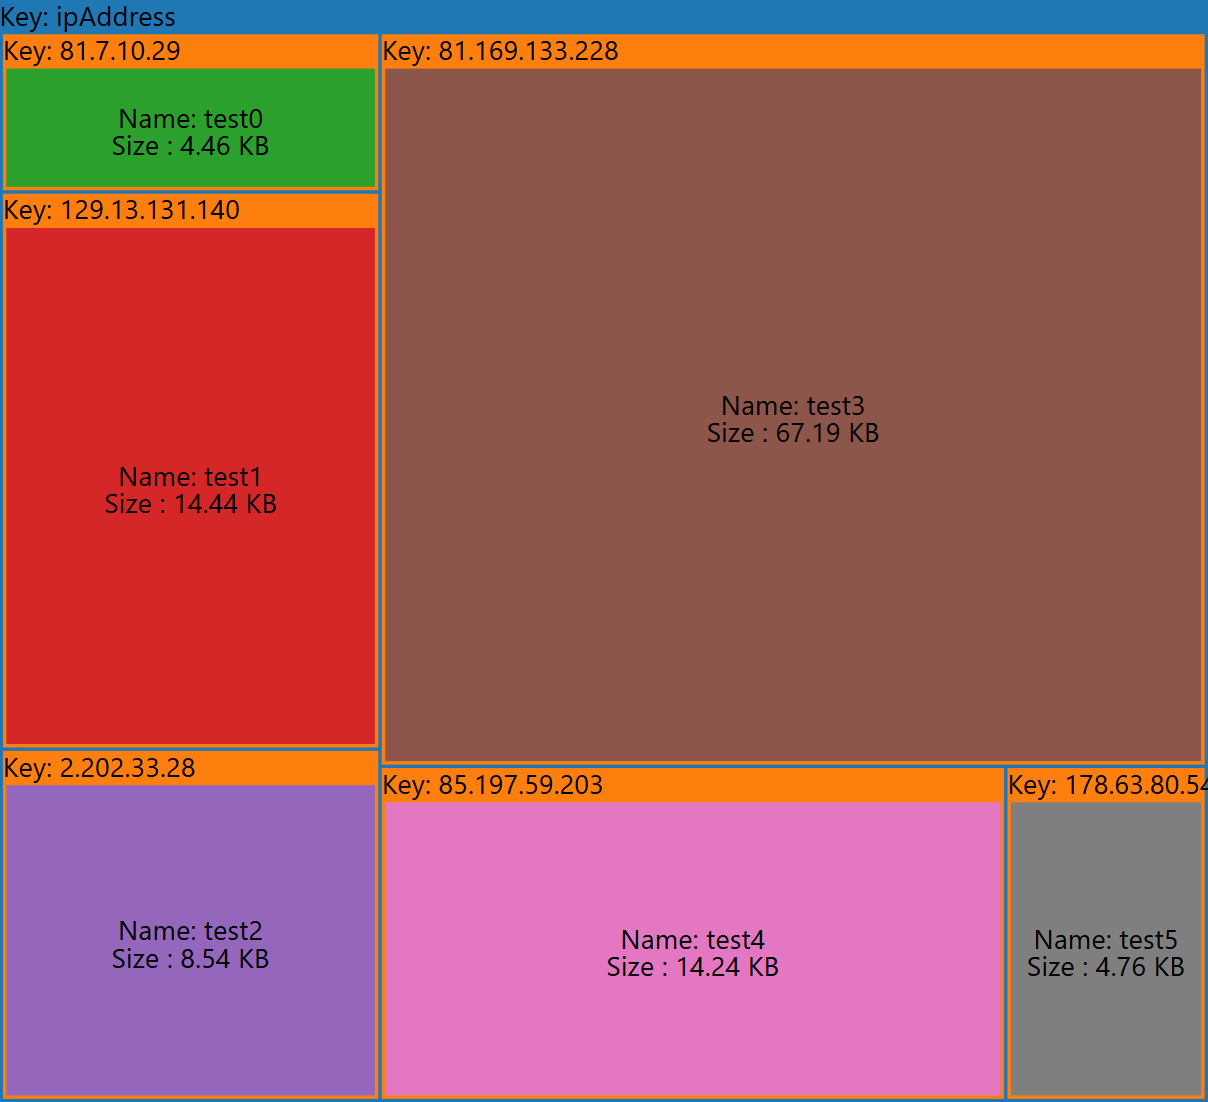
\includegraphics[width=0.7\textwidth]{../pic/IP-Tor-SetB-tree2.PNG}
\captionof{figure}{Darstellung der Beispieldaten von Alice und Bob bei der Verwendung des Tor-Netzwerks}
\label{fig:TIpTM}
\end{figure}

\begin{figure}[H]
%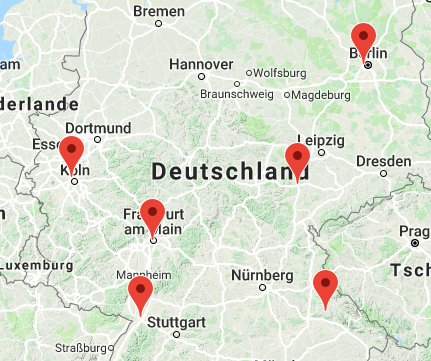
\includegraphics[width=0.7\textwidth]{../pic/IP-Tor-SetB.png}
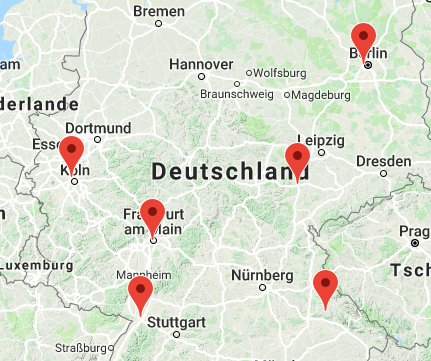
\includegraphics[width=0.4\textwidth]{../pic/IP-Tor-SetB.PNG}
\captionof{figure}{Darstellung der Beispieldaten von Alice und Bob bei der Verwendung des Tor-Netzwerks}
\label{fig:TIpM}
\end{figure}

Die Visualisierung des zweiten Falls unterscheidet sich klar von den ungeschützten Beispieldaten sowohl auch von den Beispieldaten mit Verwendung des Proxys als Methode zum Anonymisieren der Daten. 
Da jeder Datei eine anderen IP-Adresse zugeordnet ist, ist es nicht möglich anhand der IP-Adresse die Dateien den Benutzern Alice und Bob zu zuordnen.
Beide Methoden zum Anonymisieren der Daten haben somit ihre Aufgabe erfüllt und lassen eine Zuordnung der Dateien eines Benutzer zu diesem Benutzer nicht mehr zu.
\begin{comment}
    \subsection{IP-Adressen bezogene Visualisierung von Alice und Bobs Daten}

Die Darstellung von Alice und Bobs erfolgt durch eine sog. TreeMap, welche eine gegebene Datenstruktur, welche als Baum dargestellt werden kann, visualisiert.
Die Baumstruktur besteht aus einem Wurzelknoten, den davon abgehenden Kindknoten und den Blattknoten, welche dadurch ausgezeichnet sind das sie keine Kindknoten besitzen. 
Der Wurzelknoten wird künstliche erzeugt und als Überschrift für die Visualisierung verwendet und Zeigt die Schlüsseleigenschaft über dem die Baumstruktur erzeugt wurde, in diesem Fall die IP-Adresse.
Die restlichen Knoten sind aus den gegebenen Daten erzeugt worden, wobei der Schlüssel: die IP-Adresse, die Ausschlag gebende Eigenschaft ist, über welcher die Baumstruktur erzeugt wird. 
Die erzeugte Baumstruktur hat somit 3 Ebenen. 
Auf der 1. Ebene den Wurzelknoten, welche zum Visualisieren der Schlüsseleigenschaft benutzt wird. 
Auf der 2. Ebene die Kindknoten, welche die IP-Adressen darstellen, welche im Datensatz vorhanden sind und auf der 3. Ebene die Blattknoten, welche die Dateien selbst darstellen.
Für das Beispiel von Alice und Bob sieht die Baumstruktur also wie folgt aus: 

\begin{figure}[H]
\centering
	\begin{forest}
  	for tree={%
    	folder,
    	grow'=0,
    	fit=band,
  	}
  	[Schlüsseleigenschaft: IP-Adresse
  		[Alice (95.91.226.214)
			[test0]
			[test1]
			[test2]  		
  		]
  		[Bob (95.91.225.215)
			[test3]  	
  			[test4]
  			[test5]
  		]
  	]
	\end{forest}
\caption{Baumstruktur erzeugt als dem Beispiel von Alice und Bob}
\label{fig:baum}
\end{figure}

Aus dieser Struktur wird nun die TreeMap erzeugt. 
Für jeden Knoten im Baum wird ein Rechteck/Box erzeugt, dabei wird jeder Kindknoten in das Rechteck/Box des Elternknoten eingebettet. 
Durch farbliche Unterschiede sollen dann die verschiedenen Ebenen und Relationen deutlich werden. 
Eine Schematische Darstellung des Beispiels ist in~\ref{fig:schem} zu sehen. 

\begin{figure}[H]
\centering
\begin{tikzpicture}
\node (rect) [rectangle, draw, minimum width=160mm, minimum height=90mm, anchor= north west] at (0,0) {};
\node [below right] at (rect.north west) {Schlüsseleigenschaft: IP-Adresse};

\node (rectA) [rectangle, draw, minimum width=80mm, minimum height=80mm, anchor= north west] at (0,-1) {};
\node [below right] at (rectA.north west) {Alice (95.91.226.214};

\node (rectA0) [rectangle, draw, minimum width=22mm, minimum height=60mm, anchor= north west] at (0.35,-2) {};
\node [] at (rectA0.center) {test0};
\node (rectA1) [rectangle, draw, minimum width=22mm, minimum height=60mm, anchor= north west] at (2.9,-2) {};
\node [] at (rectA1.center) {test1};
\node (rectA2) [rectangle, draw, minimum width=22mm, minimum height=60mm, anchor= north west] at (5.45,-2) {};
\node [] at (rectA2.center) {test2};

\node (rectB) [rectangle, draw, minimum width=80mm, minimum height=80mm, anchor= north west] at (8,-1) {};
\node [below right] at (rectB.north west) {Bob (95.91.225.215)};

\node (rectB0) [rectangle, draw, minimum width=23mm, minimum height=60mm, anchor= north west] at (8.35,-2) {};
\node [] at (rectB0.center) {test3};
\node (rectB1) [rectangle, draw, minimum width=23mm, minimum height=60mm, anchor= north west] at (10.9,-2) {};
\node [] at (rectB1.center) {test4};
\node (rectB2) [rectangle, draw, minimum width=23mm, minimum height=60mm, anchor= north west] at (13.45,-2) {};
\node [] at (rectB2.center) {test5};
\end{tikzpicture}
\caption{Schematische Darstellung einer Visualitionmöglichkeit der Baumstruktur}
\label{fig:schem}
\end{figure}

Die Umsetztung dieses schematischen Ansatzes wird verwendet um das Beispiel von Allice und Bob darzustellen. 
Ein entsprechendes Datenbankmodell ist dafür in dem Dokumentenspeicher eingespeißt worden.

\begin{figure}[H]
%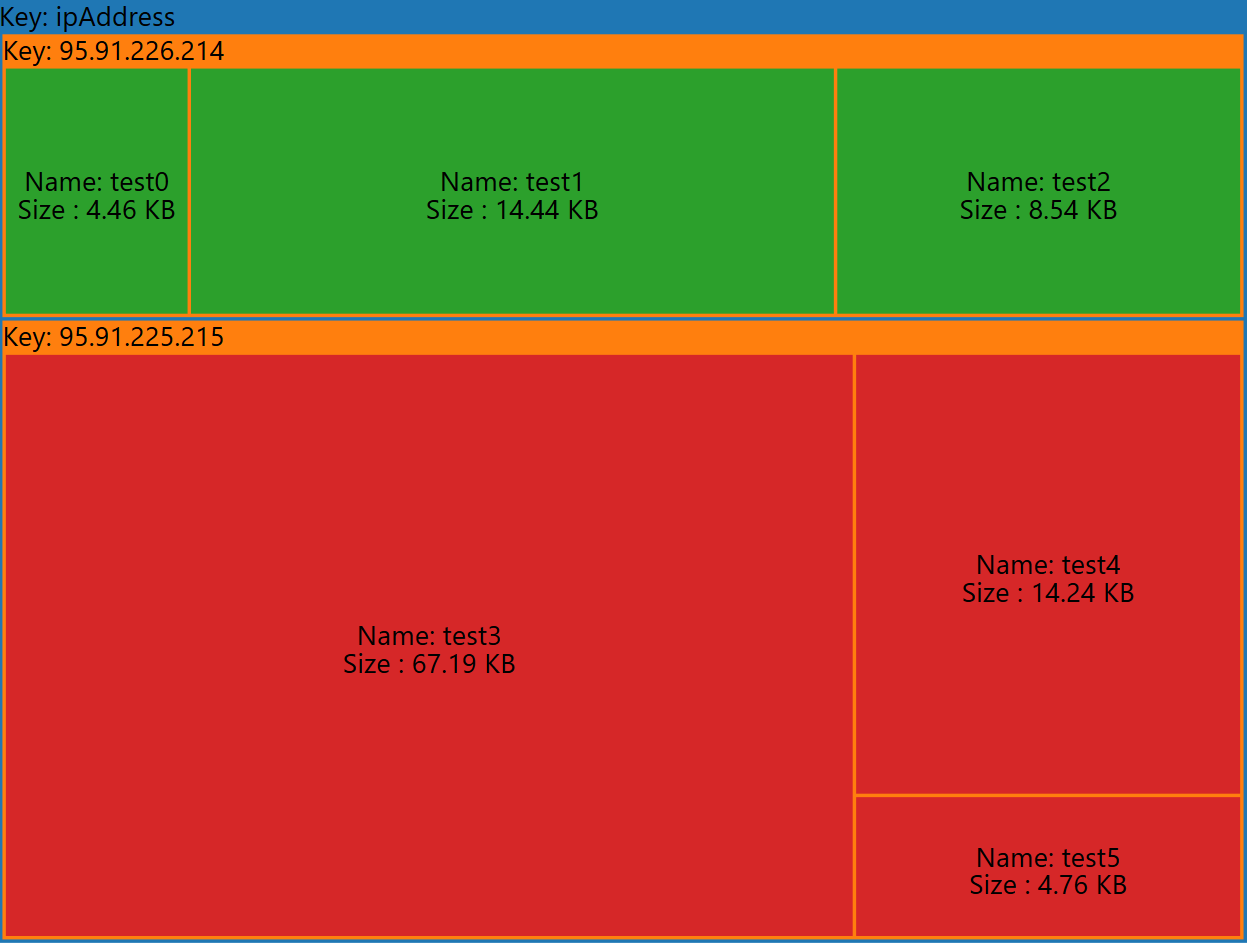
\includegraphics[width=\textwidth]{../pic/IP-Proxy-SetA-tree2.png}
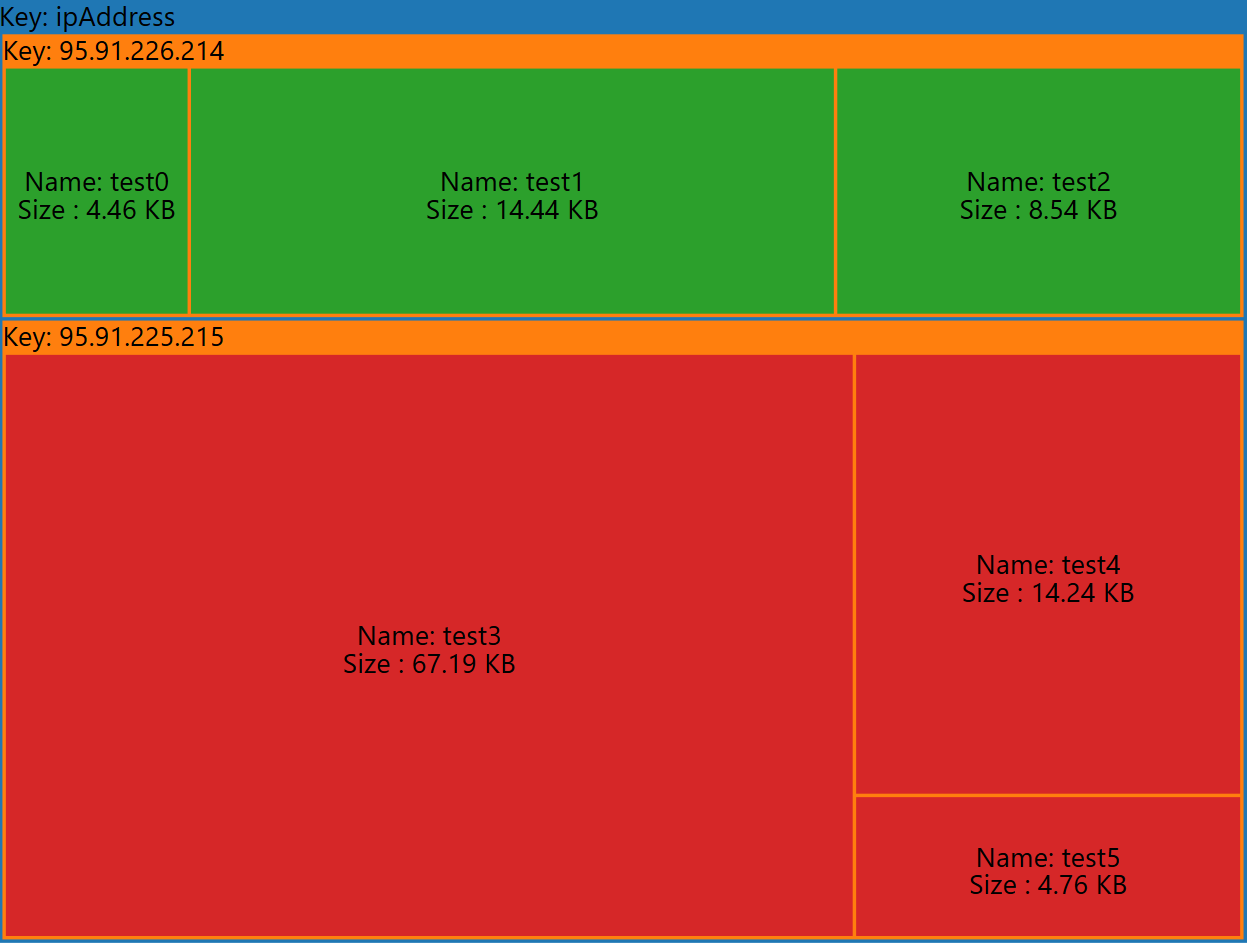
\includegraphics[width=\textwidth]{../pic/IP-Proxy-SetA-tree2.PNG}
\captionof{figure}{Darstellung der Daten von Alice und Bob}
\label{fig:tmA}
\end{figure}

In Abbildung 3.1 werden die Daten von Alice und Bob dargestellt, welche ohne die Verwendung eines Proxys hochgeladen worden sind. 

In Abbildung 3.1 sind die IP-Adressen von Alice(95.91.226.214) und Bob(95.91.225.215) erkennbar. 
Zu jeder IP-Adresse können jeweils die drei Dateien der Benutzer zugeordnet werden. 
Die Dateien test0 bis test2 sind der IP-Adresse 95.91.226.214 zugeordnet und test3 bis test5 sind der IP-Adresse 95.91.225.215 zugeordnet.
Damit ist das gegebene Beispiel richtig abgebildet und die echten Relationen zwischen Dateien und IP-Adressen sind richtig modelliert und nachvollziehbar. 

\begin{center}
%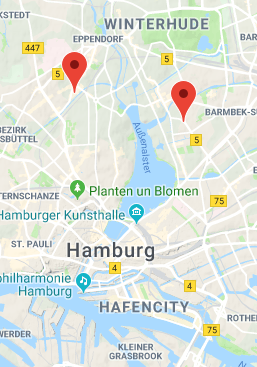
\includegraphics[width=0.5\textwidth]{../pic/IP-Proxy-SetA.png}
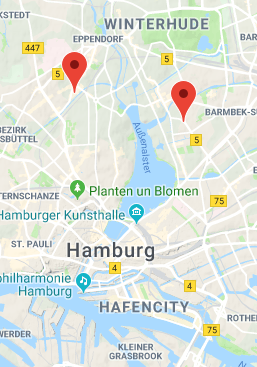
\includegraphics[width=0.5\textwidth]{../pic/IP-Proxy-SetA.PNG}
\captionof{figure}{Visualisierung von Dateien mittels einer Karte, welche die Geoposition einer IP-Adresse anzeigt}
\end{center}

Die Abbildung 3.2 zeigt uns die Geoposition der IP-Adressen von Alice und Bob und zeigt deren Position in Hamburg, 
wobei die Position nur einen ungefähren Standpunkt darstellt und die eigentliche Position bis zu einem Kilometer abweichen kann.

\begin{center}
%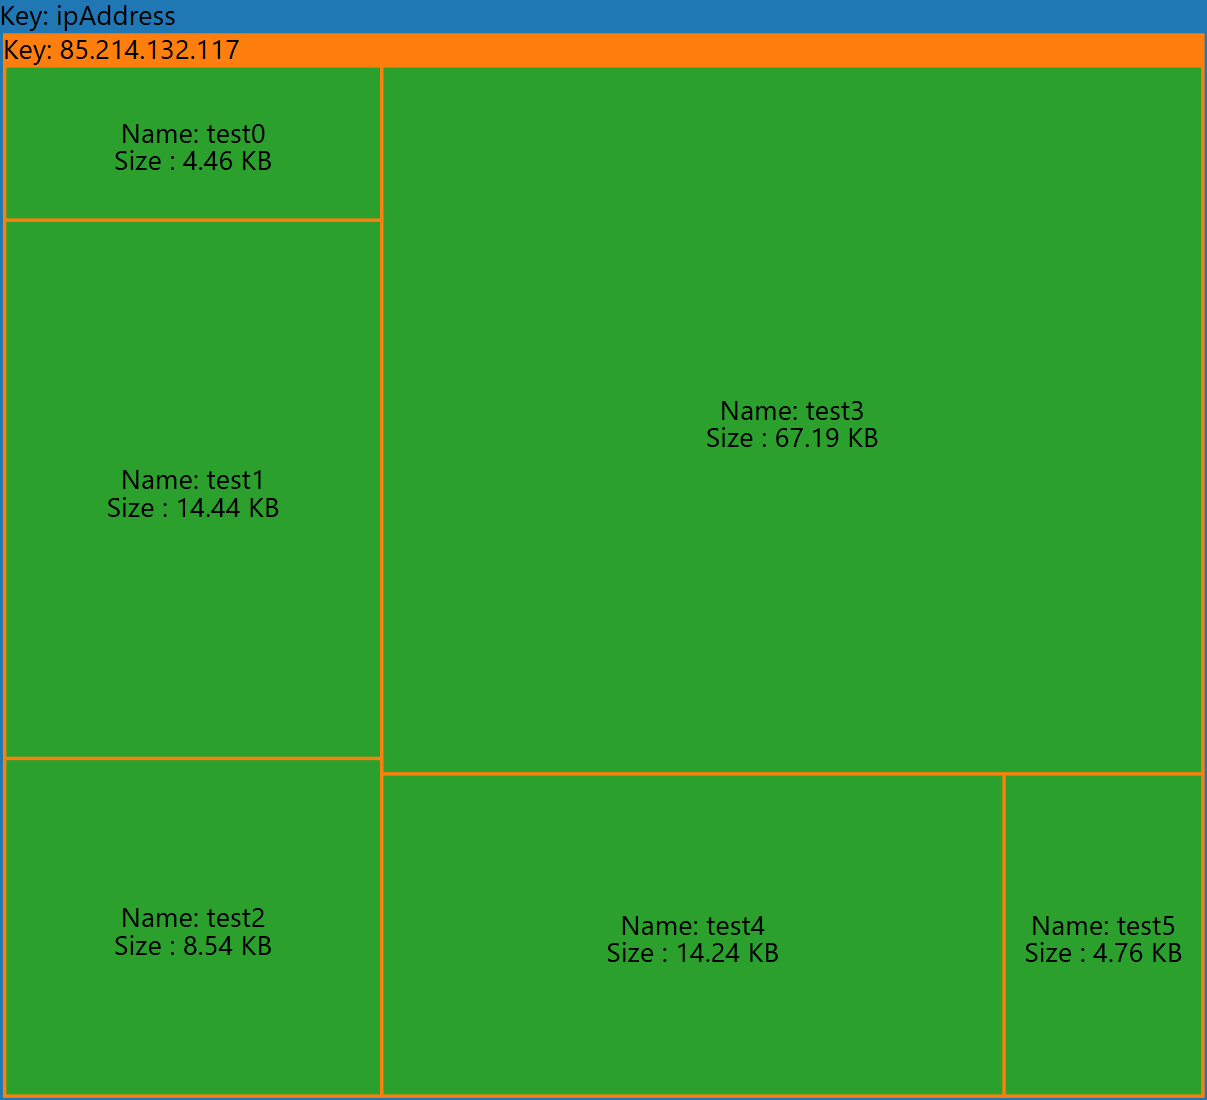
\includegraphics[width=\textwidth]{../pic/IP-Proxy-SetB-tree2.png}
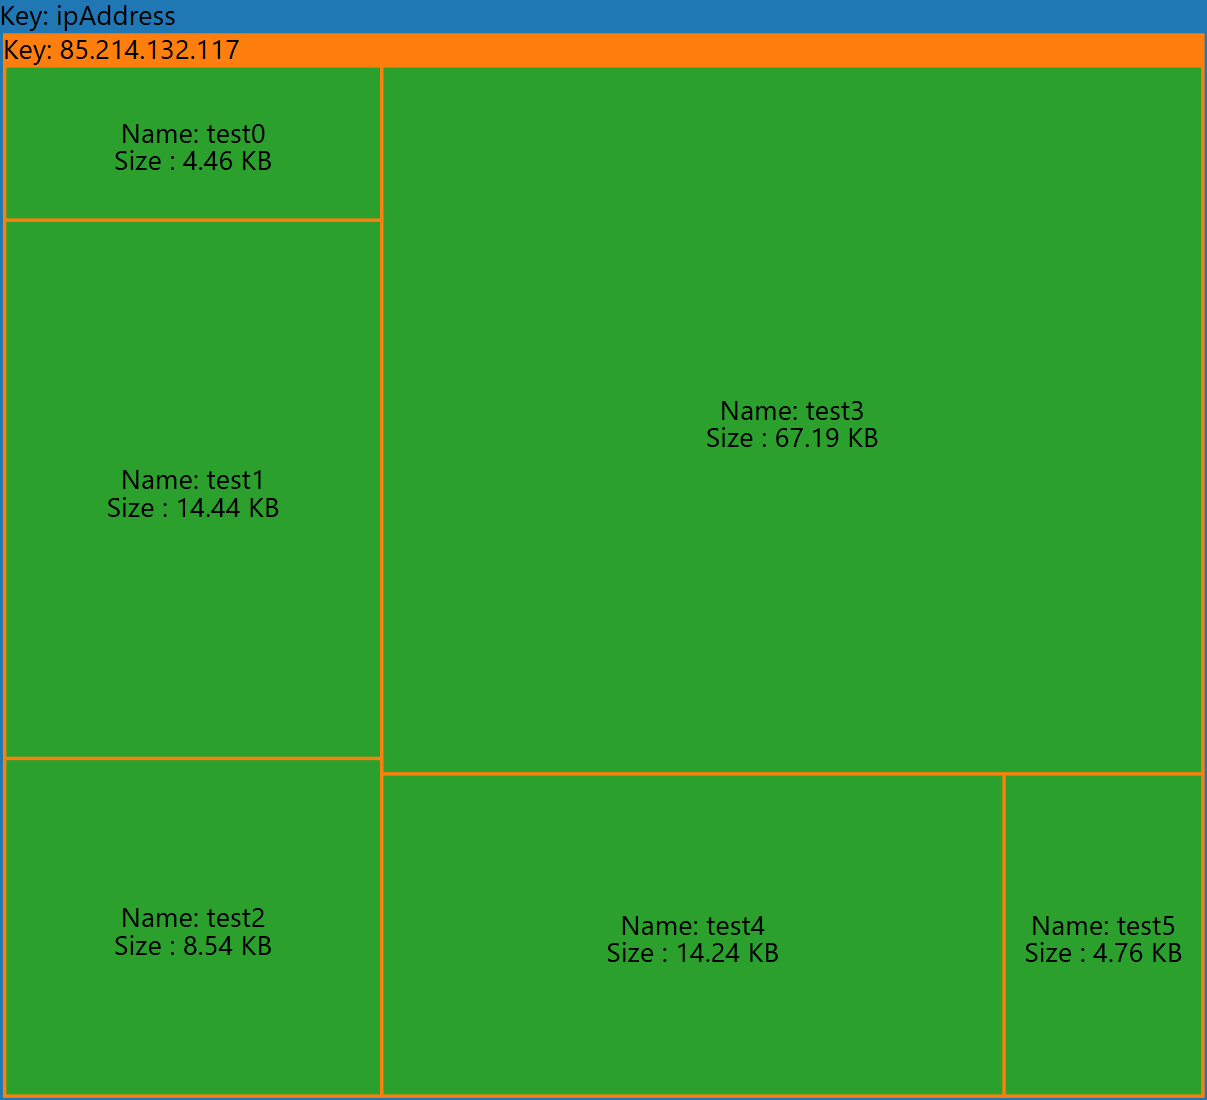
\includegraphics[width=\textwidth]{../pic/IP-Proxy-SetB-tree2.PNG}
\captionof{figure}{Visualisierung von Dateien mittels einer TreeMap, welche nach der IP-Adresse gruppiert sind}
\end{center}

In Abbildung 3.3 sind die Daten visualisiert, welche mittels eines proxy hochgeladen wurden. 
Alle Dateien wurden über die IP-Adresse des proxys 85.214.132.117 gruppiert und somit eine Anonymitätsmenge erzeugt.
Die Daten von Alice und Bob sind nun in einer Anonymitätsmenge zusammengefasst und lassen sich anhand der IP-Adresse nicht mehr eindeutig den beiden Benutzern zuordnen.

\begin{center}
%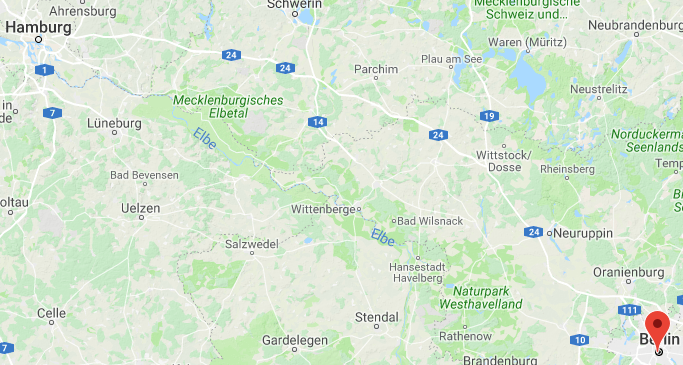
\includegraphics[width=\textwidth]{../pic/IP-Proxy-SetB.png}
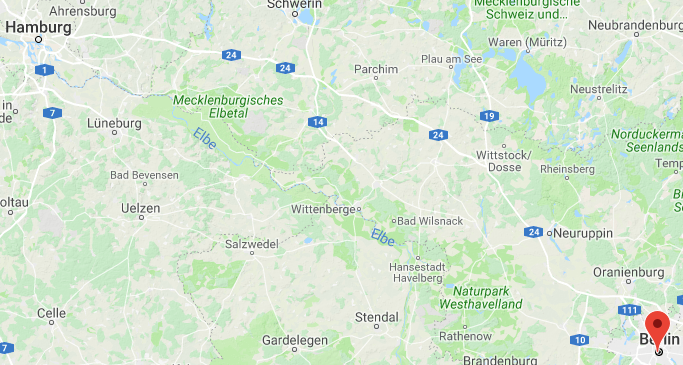
\includegraphics[width=\textwidth]{../pic/IP-Proxy-SetB.PNG}
\captionof{figure}{Visualisierung von Dateien mittels einer Karte, welche die Geoposition einer IP-Adresse anzeigt}
\end{center}

Abbildung 3.4 zeigt und nun die Geoposition des proxys welches in Berlin steht.
Damit sind auch die eigentlichen Geoposition von Alice und Bob durch die Verwendung des Proxys maskiert worden. 

Anstelle eines proxys könnten Alice und Bob das Tor-Netzwerk benutzen um ihre IP-Adressen zu maskieren. Alice und Bob laden drei Dateien, einmal ungeschützt und einmal geschützt durch das Tor-Netzwerk hoch.
Dabei nehmen wir an das alle Dateien einzeln hochgeladen wurden und jeder hochgeladenen Datei eine andere Route durch das Tor-Netzwerk zugewiesen wurde, sodass jede hochgeladene Dateie einen anderen Exit-Server des Tor-Netzwerkes durchläuft. 

\begin{center}
%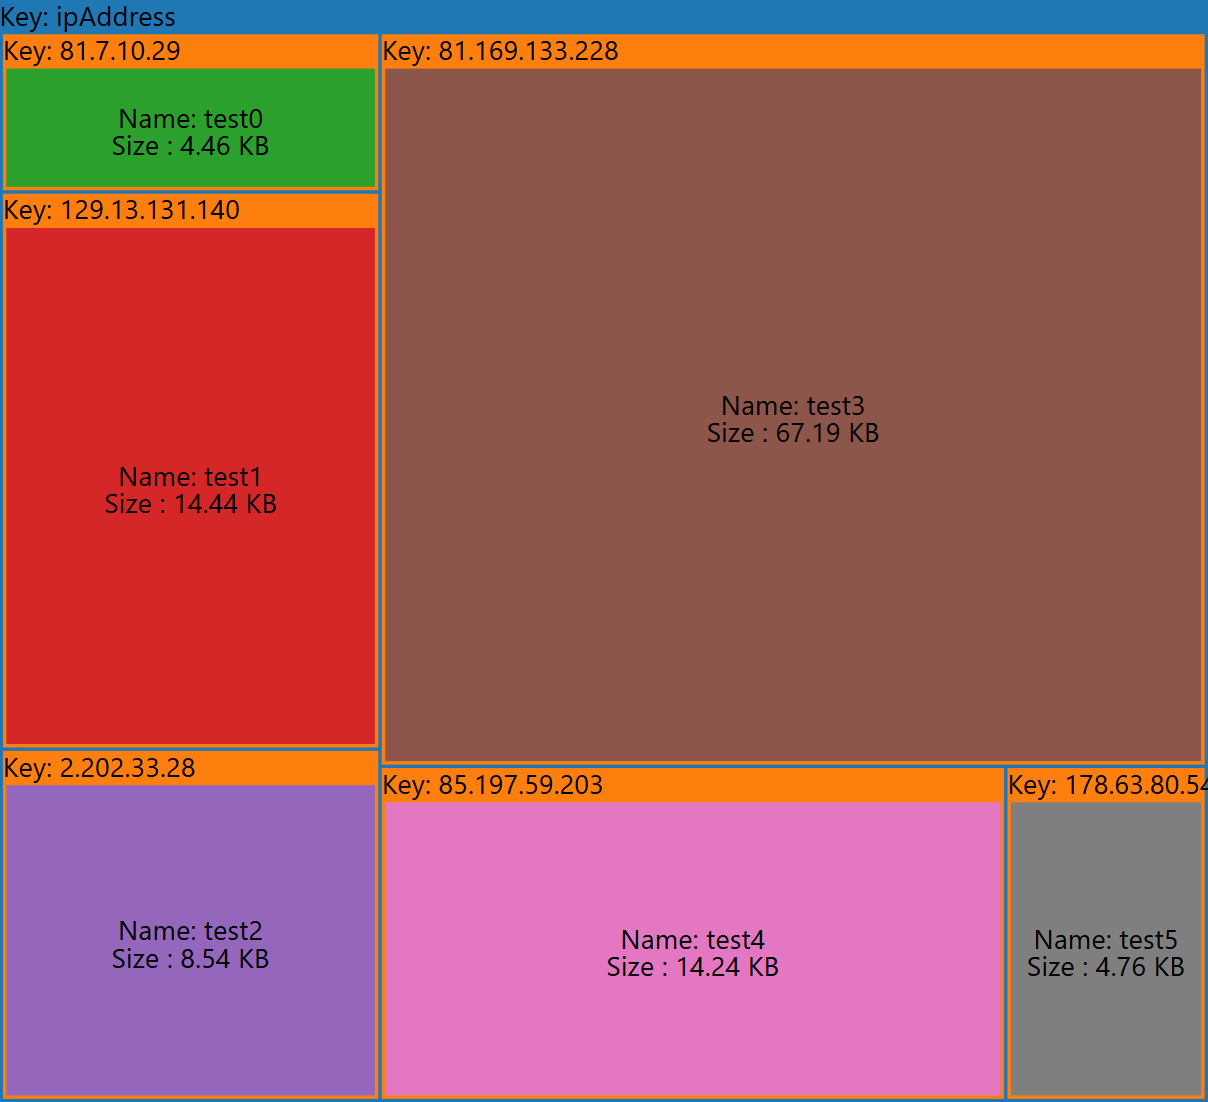
\includegraphics[width=\textwidth]{../pic/IP-Tor-SetB-tree2.png}
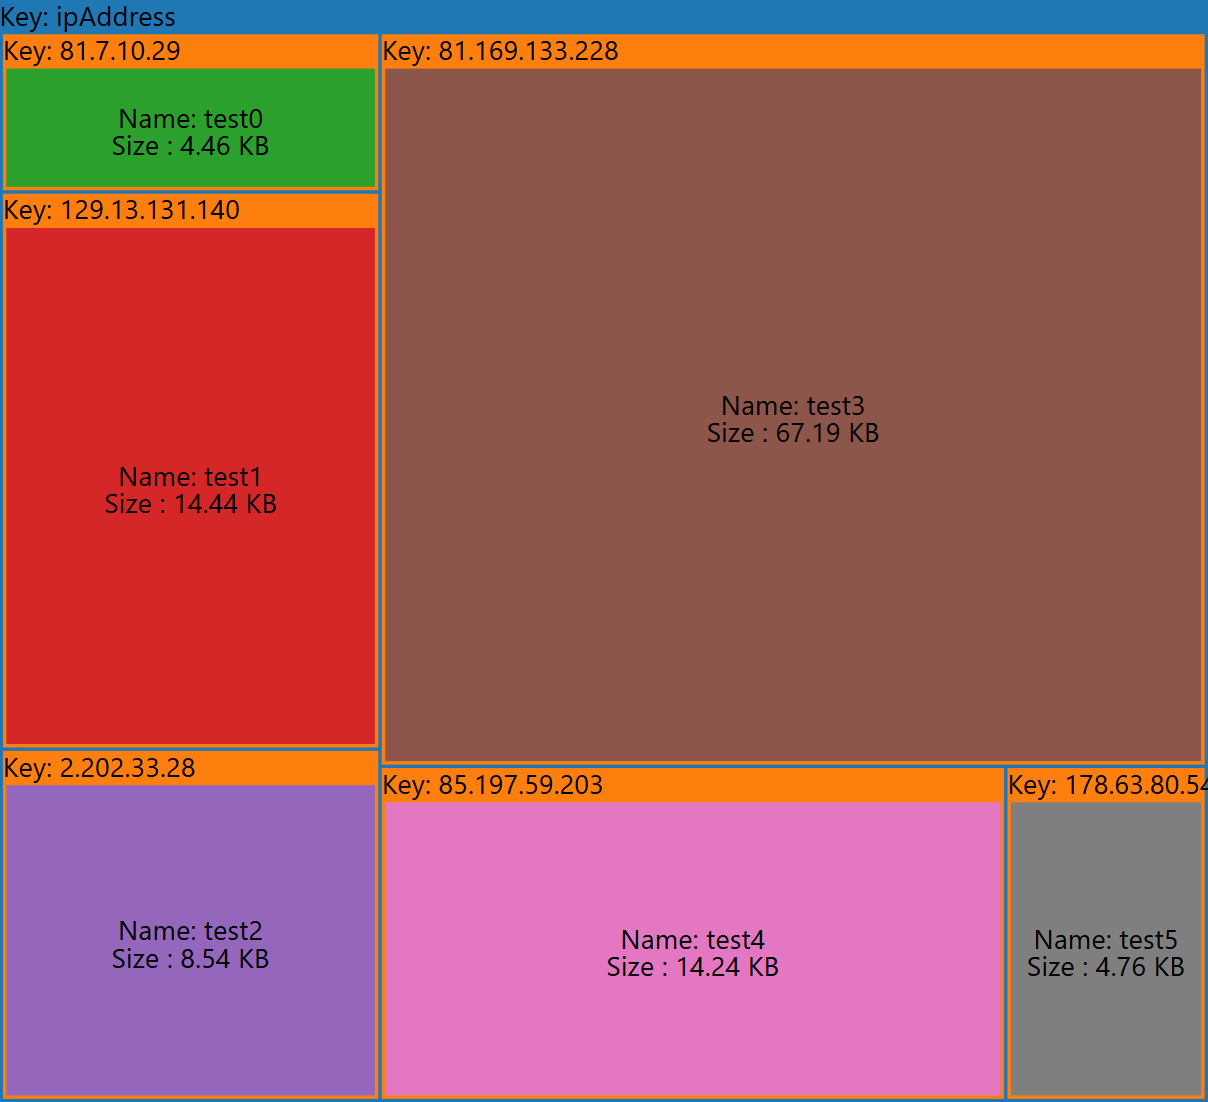
\includegraphics[width=\textwidth]{../pic/IP-Tor-SetB-tree2.PNG}
\captionof{figure}{Visualisierung von Dateien mittels einer TreeMap, welche nach der IP-Adresse gruppiert sind}
\end{center}

In Abbildung 3.5 sehen wir nun die IP-Adressen der verschiedenen Exit-Server des Tor-Netzwerks.
Da jeder hochgeladener Datei ein neuer Exit-Server zugewiesen wurde, können wir über die IP-Adresse die Dateien nicht mehr entsprechend der Benutzer gruppieren.

\begin{center}
%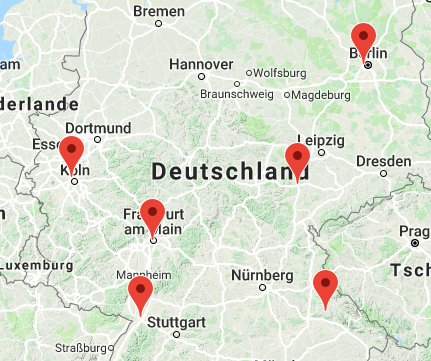
\includegraphics[width=0.7\textwidth]{../pic/IP-Tor-SetB.png}
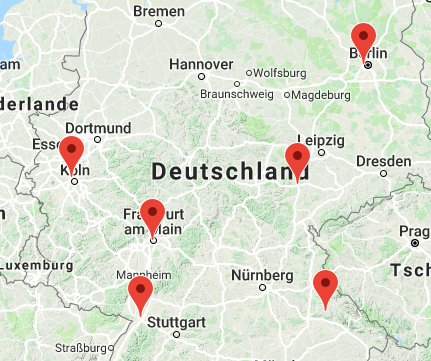
\includegraphics[width=0.7\textwidth]{../pic/IP-Tor-SetB.PNG}
\captionof{figure}{Visualisierung von Dateien mittels einer Karte, welche die Geoposition einer IP-Adresse anzeigt}
\end{center}

Bei Betrachtung der Abbildung 3.6 ist auch erkennbar, das die verschiedenen Positionen der Exit-Server des Tor-Netzwerks variieren und es keinen Anhaltspunkt auf die eigentliche Postion von Alice und Bob gibt. 
\end{comment}

\newpage
    \subsection{Darstellung: Headerfingerprinting}
Der Headerfingerprint wird wie im Kapitel~\ref{ipVis} beschrieben mit einer sog. TreeMap und einer dieser TreeMap zugrundeliegender Baumstruktur.
Nur die Schlüsseleigenschaft wird für diese Visualisierung von der IP-Adresse auf den Headerfingerprint geändert.
Für die ungeschützten Beispieldaten von Alice und Bob erhalten wir die Visualisierung nach Abbildung~\ref{fig:ungHTM}.
Zusehen ist der Headerfingerprint von Alice mit zugeordneten Dateien test0, test1 und test2, sowie den Headerfingerprint von Bob mit den zugeordneten Dateien test3, test4 und test5.

\begin{figure}[H]
%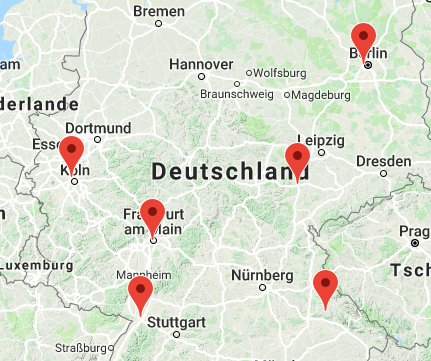
\includegraphics[width=0.7\textwidth]{../pic/IP-Tor-SetB.png}
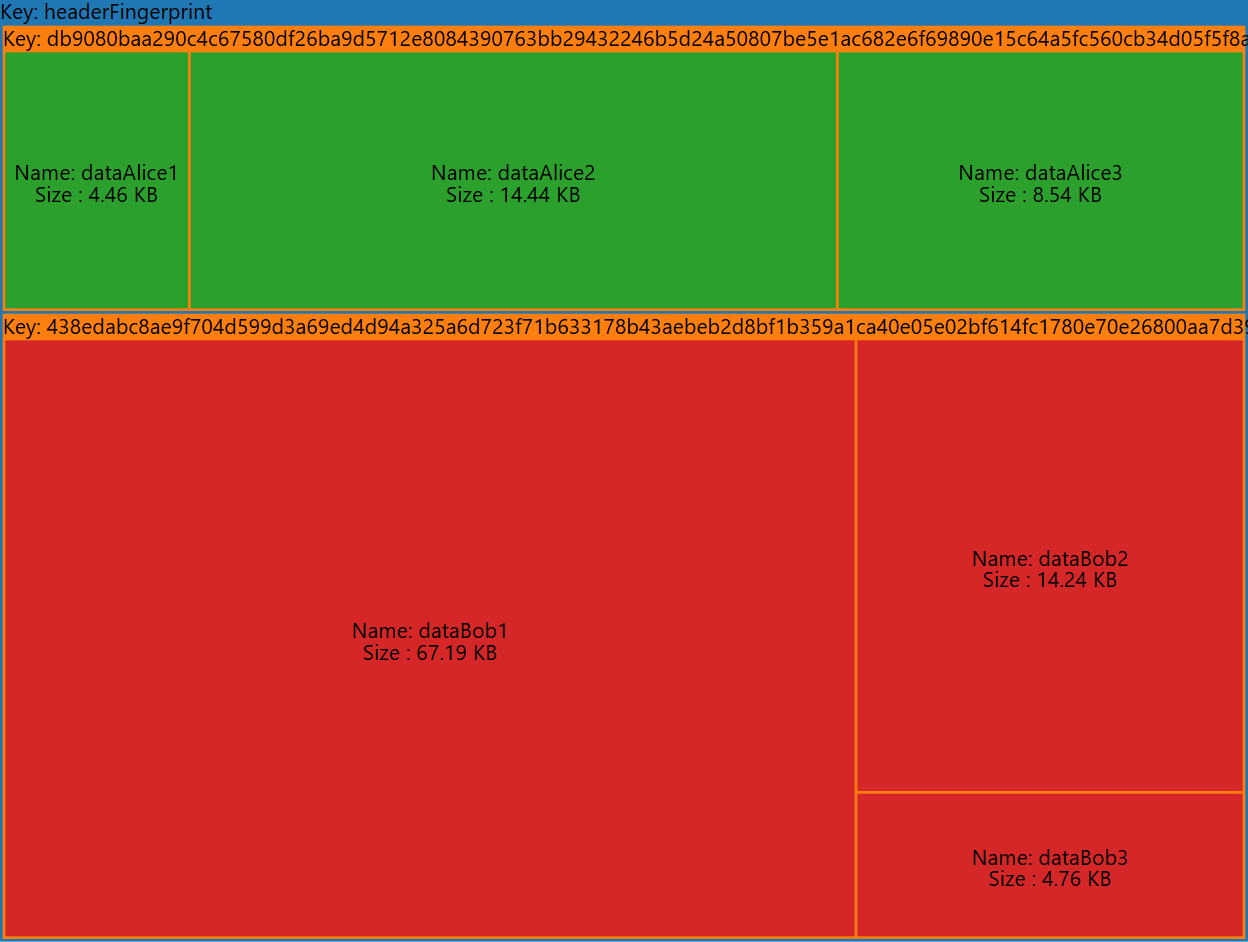
\includegraphics[width=0.7\textwidth]{../pic/Header-Proxy-SetA.PNG}
\captionof{figure}{Darstellung der Beispieldaten von Alice und Bob bei der Verwendung eines Proxy}
\label{fig:ungHTM}
\end{figure}

Wie in Abbildung~\ref{fig:ungIpTM} stellt Abbildung~\ref{fig:ungHTM} die Relationen der Beispieldaten und Benutzer richtig dar. 

Bei Betrachtung der Visualisierung der Beispieldaten bei der Verwendung eines Proxys erhalten wir die Visualisierung nach Abbildung~\ref{fig:PHTM}.
Diese Visualisierung ist mit der Visualisierung der ungeschützten Beispieldaten in Abbildung~\ref{fig:ungHTM} identisch. 
Der Headerfingerprint von Alice ist dargestellt sowie die Dateien von Alice test0, test1 und test2 sind diesem Headerfingerprint zugeordnet.
Der Headerfingerprint von Bob ist ebenfalls dargestellt und die Beispieldateien von Bob test3, test4 und test5 sind diesem zugeordnet.

\begin{figure}[H]
%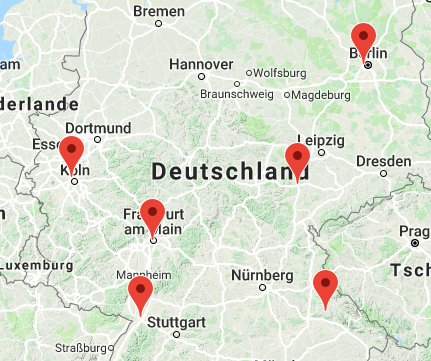
\includegraphics[width=0.7\textwidth]{../pic/IP-Tor-SetB.png}
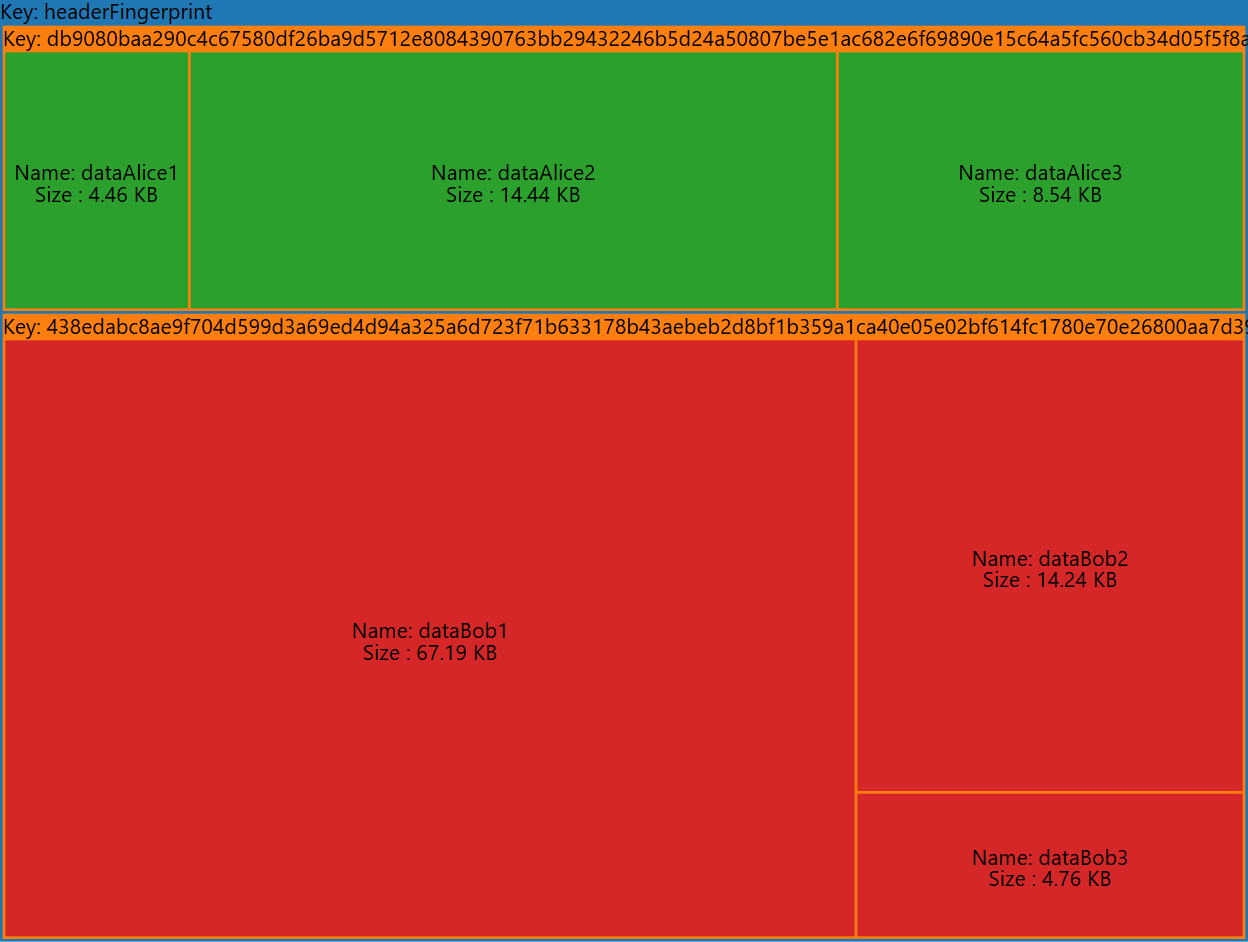
\includegraphics[width=0.7\textwidth]{../pic/Header-Proxy-SetA.PNG}
\captionof{figure}{Darstellung der Beispieldaten von Alice und Bob bei der Verwendung eines Proxy}
\label{fig:PHTM}
\end{figure}

Bei Betrachtung des zweiten Falls der Verwendung des Tor-Netzwerkes entspricht die Visualisierung der Abbildung~\ref{fig:THTM}.
Zu erkennen ist das ähnlich der Abbildung~\ref{fig:PIpTM} alle Dateien unter einem Headerfingerprint angeordnet sind.
Header-Tor-SetB.png
\begin{figure}[H]
%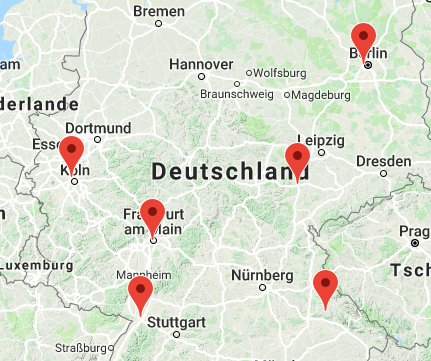
\includegraphics[width=0.7\textwidth]{../pic/IP-Tor-SetB.png}
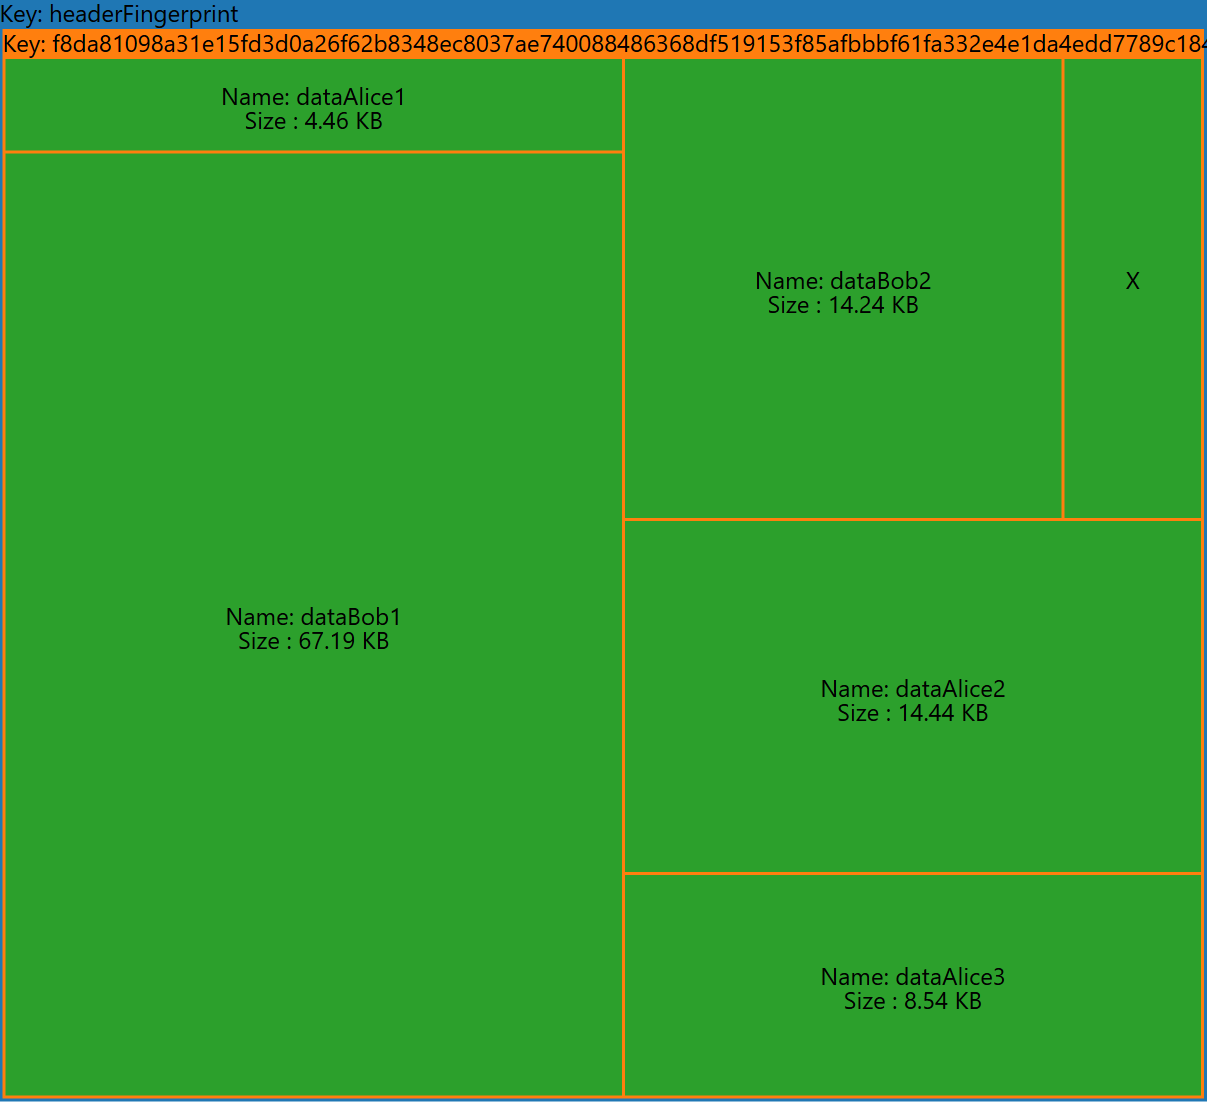
\includegraphics[width=0.7\textwidth]{../pic/Header-Tor-SetB.png}
\captionof{figure}{Darstellung der Beispieldaten von Alice und Bob bei der Verwendung des Tor-Netzwerkes}
\label{fig:THTM}
\end{figure}

Die Verwendung das Tor-Netzwerks hat somit eine Anonymitätsmenge für die Eigenschaft des Headerfingerprints erzeugt, in welcher Menge die Dateien Anonym sind und den Benutzern Alice und Bob nicht zugeordnet werden können.

Somit ist klar erkennbar das die Verwendung eins Proxys keine Auswirkung auf die übermittelten Header hatte und Alice und Bob trotz der Verwendung eines Proxys an ihren spezifischen Headern in diesem Beispiel identifiziert werden können.
Die Verwendung des Tor-Netzwerks, jedoch erzeugt eine Anonymitätsmenge über dem Headerfingerprint, durch welche die Dateien Anonymisiert werden.
Die Verwendung des Proxys zeigt hier somit bereits eine Schwäche gegenüber der Verwendung der Tor-Netzwerks auf, sie nur Schutz vor der Zuordnung der Dateien im Hinblick auf die IP-Adresse gibt.
Nicht jedoch im Hinblick auf den Headerfingerprint.
Die Verwendung des Tor-Netzwerks schützt sowohl vor der Erkennnung der Relationen von Benutzern und Dateien im Bezug auf die IP-Adresse sowohl auch der des Headerfingerprint.




% Schluss
\chapter{Schluss}
\section{Zusammenfassung der Ergebnisse}
\section{Limitierungen}
\section{Ausblick}
\end{document}
